% Lua(La)TeX-Dokument! Kodierung: Unicode, UTF-8. Schriftart: Linux Libertine Normal, Schriftgröße 12. Druck auf DIN A4, beispielsweise als Ringbindung zum einfachen Herausnehmen einzelner Seiten.

\begin{filecontents*}{0-infiniteadventures-bonusband-current.xmpdata}
    \Title{Infinite Adventures: Bonusband}
    \Author{Mirco Hensel, yury und Tobias Frei, infiniteadventures.de}
    \Copyright{Mirco Hensel, yury und Tobias Frei, infiniteadventures.de}
    \Org{infiniteadventures.de}
    \PublicationType{book}
    \Keywords{German\sep bonus material\sep freely licensed\sep open source}
    \Subject{Der Bonusband zum Roman "Infinite Adventures". Open Source, geschrieben in LaTeX (LuaTeX).}
\end{filecontents*}
% Nach Änderungen am xmpdata-Abschnitt muss die ".xmpdata"-Datei manuell gelöscht werden.

\documentclass[paper=a4,pagesize=auto,fontsize=12pt,div=13,BCOR=15mm]{scrbook}
% Dabei gilt:
% 	A5 ist die Papiergröße,
%	pagesize=auto
% 	12pt ist die Schriftgröße,
% 	div=13 beeinflusst unter Anderem die Randgröße. Einen perfekten Wert gibt es nicht.
% 	BCOR=15mm fügt 15 Millimeter Bindekorrektur an den Innenrändern hinzu.

%\usepackage{colorprofiles}
% "sRGB_IEC61966-2-1_black_scaled.icc"-Farbprofil für das "pdfx"-Paket
% Wird nicht benötigt, da wir das frei lizenzierte Farbprofil einfach als ".icc"-Datei mitliefern.
% Falls die Datei fehlen sollte, genügt es nicht, diese Zeile auszukommentieren.
% Die im Paket "colorprofiles" enthaltene Datei müsste zudem umbenannt werden,
% sonst wird sie nicht gefunden. ("sRGB_IEC61966-2-1_black_scaled.icc")
% Noch ein Fallstrick:
% Manche Dateisysteme unterscheiden zwischen Groß- und Kleinschreibung.

\usepackage[a-1b]{pdfx}
% "PDF-A/1-b"-Standard einhalten; Konformität in den PDF-Metadaten ankündigen und einfordern.

\usepackage{hyperref}
% Verlinkung im Inhaltsverzeichnis.
% Enthalten in "pdfx", daher OHNE ZUSATZOPTIONEN wie "hidelinks", sonst gibt es eine Fehlermeldung.

\hypersetup{
    colorlinks=false,
    pdfborder={0 0 0},
}
% pdfx-kompatible Alternative zu "hidelinks":
% Links nicht in bunter Schrift darstellen, keine roten Kästen um Links darstellen.

\usepackage{polyglossia}
% Das hieß früher "babel". Polyglossia ist der Nachfolger.

\setdefaultlanguage[spelling=new, babelshorthands=false]{german}
% Neue deutsche Rechtschreibung,

\usepackage{fontspec}
\usepackage{unicode-math}
% Ein paar wenige Szenen verwenden mathematische Formeln.

\setromanfont{Linux Libertine}
\setsansfont{Linux Biolinum}
\setmonofont{Linux Libertine Mono}
\setmathfont{STIX Two Math}
% ausschließlich frei lizenzierte Schriften

\usepackage{microtype}
% Zeilenränder glätten durch minimal veränderte Buchstabenabstände (Blocksatz).
% Dabei wird nicht mathematisch exakt eine Randlinie gezogen,
% sondern der optische Eindruck beachtet.
% "Löcher" durch Punkte und Bindestriche am rechten Rand werden vermieden,
% indem diese Zeichen ein kleines Stück über den Rand hinaus geschoben werden.

\usepackage{graphicx}
% Einbinden von Bildern. PDF ist dabei ein gültiges Bildformat.

\usepackage{pdfpages}
% Einbinden von PDF-Seiten als 1:1-Kopie, wenn Verkleinerung nicht gewünscht ist

\setlength{\emergencystretch}{2em}
% Der Blocksatz darf auch größere Leerzeichen (bis zu 2 em breit) enthalten.

\typearea[15mm]{13}
% Sehr wichtig: Der Seitenrand muss nach dem Laden aller Schriftarten neu berechnet werden.
% 15mm sind die Bindekorrektur, 13 ist der DIV-Wert.
% Mehr DIV = kleinere Ränder.

\begin{document}

\pagestyle{plain}
% Keine Kapitelüberschrift in der Kopfzeile; nur Seitenzahlen in der Fußzeile.

\extratitle{\textbf{Infinite Adventures: Bonusband}\\Originale deutschsprachige Fassung – nicht übersetzt.\\© Mirco Hensel, yury und Tobias Frei, infiniteadventures.de

\bigskip

\noindent Dies ist eine offizielle Ausgabe des Infinite-Adventures-Bonusbands, herausgegeben von Tobias Frei. Veränderte Versionen und unautorisierte Nachdrucke müssen deutlich als solche gekennzeichnet werden. Auch das Impressum muss angepasst werden, wenn das Dokument verändert wird.

\bigskip

DIESES DOKUMENT IST NOCH NICHT FERTIG. DIE LIZENZ IST NOCH NICHT GÜLTIG. WÄHREND DIESER ÜBERARBEITUNGSPHASE GILT: ALLE RECHTE VORBEHALTEN. DIE VERÖFFENTLICHUNG IST UNGEFÄHR FÜR AUGUST 2018 GEPLANT. DIESER ABSATZ WIRD VOR DER VERÖFFENTLICHUNG ENTFERNT.

\noindent Printed on Örz, NGC 6193 – brought to you by IGLS, your friendly interstellar freight forwarding service!}

\title{Infinite Adventures: Bonusband}

\subtitle{»Unterschätze niemals dein Haustier.\linebreak[3] Es könnte dein Raumschiff klauen.«}
%Ein Zeilenumbruch wird nicht erzwungen, aber vorgeschlagen (Priorität 0-4).

\author{Mirco Hensel, yury und Tobias Frei,\\ infiniteadventures.de}

\date{} % Ein "leeres Datum" entfernt die Datumsangabe auf der Titelseite.

\dedication{in Erinnerung an Douglas Adams}

\lowertitleback{\noindent Texte: © Mirco Hensel, yury und Tobias Frei,\\ infiniteadventures.de

\bigskip

\noindent Der gesamte Inhalt des Bonusbands ist frei lizenziert; Bildquellen und Lizenzen sind am Ende des Buches abgedruckt. Solange es die offizielle Website gibt, kann das gesamte Material inklusive LaTeX-Quelltext dort heruntergeladen werden. Außerdem findest Du wahrscheinlich auf Internetportalen wie dem Internet Archive, GitHub, Wikimedia Commons etc. die entsprechenden Dateien. Wir freuen uns, wenn Du die Möglichkeiten der Lizenz nutzt und die Infinite Adventures in der Welt verbreitest.

\bigskip

\noindent Dieses Dokument enthält Internetlinks, die zum Zeitpunkt der Veröffentlichung von mir geprüft wurden. Den Inhalt der verlinkten Seiten mache ich mir allerdings nicht zu eigen; ich habe keine Kontrolle über spätere Veränderungen des verlinkten Inhalts. Sollte entgegen meiner Erwartungen eines Tages ein Link defekt oder sogar schädlich bzw. unangemessen geworden sein, bitte ich um eine Benachrichtigung per Post. Ich werde solche Links dann schnellstmöglich aus weiteren Ausgaben entfernen. Da ich keine Haftung für die Sicherheit der Links übernehmen kann, erfolgt das Aufrufen der verlinkten Seiten auf eigene Gefahr.

\bigskip

\noindent Die Deutsche Nationalbibliothek verzeichnet diese Publikation in der Deutschen Nationalbibliografie; detaillierte bibliografische Daten sind im Internet über http://dnb.dnb.de abrufbar.

\bigskip

\noindent ISBN: 000-0-00000-000-0\\ Erste Auflage, 2018

\noindent Verlag \& Herausgeber:\\
\noindent Tobias Frei\\
\noindent Böhler Weg 19\\
\noindent 42285 Wuppertal\\
\noindent tobias@tfrei.de

\noindent Druck: epubli – ein Service der neopubli GmbH, Berlin}

\maketitle

\tableofcontents

	\newpage

\part{Texte}

\chapter{Vorwort}

Dieser Bonusband ist als Ergänzung zum Roman »Infinite Adventures« von Mirco Hensel, yury und Tobias Frei erstellt worden. Er soll offene Fragen klären, solange diese nicht sowieso in einem Fortsetzungsband beantwortet werden. Außerdem enthält dieser Bonusband einige Fotos und Darstellungen, die im kleinen DIN-A5-Buchformat nicht vollständig zur Geltung kommen konnten.

Die Fotos werden, soweit möglich, ganzseitig und randlos gedruckt. Damit man die schönen Bilder heraustrennen kann, ohne den Bonusband zu zerstören, ist jedes Bild dreimal vorhanden. Die Rückseite der Bilder wurde absichtlich nicht bedruckt. Es bietet sich beispielsweise an, jeweils zwei Exemplare herauszunehmen und in passenden Bilderrahmen an eine Wand zu hängen. Alternativ könnten die Motive als Vorderseite selbst gebastelter Postkarten oder Lesezeichen genutzt werden. Der dreifache Druck ist ein Versuch, die dabei entstehenden Kosten möglichst gering zu halten: Wenn ein Bild zu selten vorhanden ist, müsste man den gesamten Bonusband noch einmal kaufen, um weitere Exemplare zu erhalten. Wenn die Bilder zu häufig gedruckt werden, steigen die Druckkosten für jeden Bonusband an, und man hält für einen vollkommen übertriebenen Preis zwanzig Kopien eines gar nicht gewünschten Bildes in den Händen.

Falls Dir der Bonusband zum tieferen Eintauchen in die Welt der Infinite Adventures noch nicht genügt, werden auf der offiziellen Website hoffentlich sämtliche Bilddateien zum Download angeboten. Nicht alle Bilder sind groß genug dafür, aber die größten Exemplare sähen möglicherweise auch auf DIN-A3-Aluminium-Verbundplatten gut aus. Die Autoren haben in diesem Bereich nicht die nötige Erfahrung, um eine Empfehlung abgeben zu können; es handelt sich hierbei um einen Denkanstoß, der als Grundlage für eine intensive Recherche dienen könnte.

Zudem existiert hoffentlich, während Du dieses Vorwort liest, ein sogenanntes »Wiki« zu den Infinite Adventures, welches auf der offiziellen Website von den Autoren persönlich verwaltet wird.


\chapter{Ein Roman ohne Einleitung?}

\begin{center}
    \textbf{Einleitungen sind langweilig.}
\end{center}

Die Charaktereigenschaften der Protagonisten haben sich erst beim Schreiben, also im Verlauf der Geschichte, entwickelt. Zudem wurde das Alter der Protagonisten ganz bewusst nirgendwo genannt. Dass Alexandra als "Mädchen" bezeichnet wird, schließt bei näherer Überlegung einen ziemlich großen Altersbereich ein. Allzu jung wird die Sprengstoffexpertin wohl nicht sein, auch nicht über 40 Jahre alt. Das ergibt sich durch Überlegungen beim Leser, der sich die Protagonisten so vorstellen kann und soll, wie er möchte. 

Wenn in der Fantasie des Protagonisten vier geniale Schulkinder mit Helikoptern um die Welt fliegen, ist das genauso plausibel wie die Vorstellung, es seien junge Studenten. Vielleicht sind es ja sogar Erwachsene in einer Midlife-Crisis.

Der Leser wird genau wie die Autoren damals in die Geschichte hinein geworfen. Eine Einleitung vor dieser etwas ungewöhnlichen Geschichte führt nur dazu, dass manche Leser das Buch zu Unrecht weglegen und nicht mehr weiterlesen. Jede halbwegs klassische Einleitung würde den Charakter des Buches beschädigen und den Infinite Adventures einen Reiz nehmen, der sie von anderen Geschichten unterscheidet.


\chapter{Free hackt den FBI-Server}

\textit{»Wir brechen aus dem Kindergarten aus«, entschied yury. »Dieses tolle idiotensichere Programm baut doch im Hintergrund bestimmt eine Verbindung auf, die du nachverfolgen kannst.«}

\bigskip

Innerhalb weniger Minuten dringen yury und Free aus einem Langstreckenflugzeug über dem Atlantik in das interne Netzwerk der amerikanischen Bundespolizei ein und stehlen mit absurd wirkender Leichtigkeit eine streng geheime Datenbank. Dabei läuft laut Musikliste ein Song im Hintergrund, dessen Refrain mit »Feel good – like a tiger« den Eindruck eines gemütlichen Sonntagsspaziergangs noch verstärkt.

Das ist nicht die Art von Hacking-Szene, die man aus schlechten Filmen kennt; kein großer, plakativer \textit{»Hacking in progress«}-Ladebalken kriecht untermalt von dramatischer Musik unter Zeitdruck auf die 100-Prozent-Marke zu. Technisch wenig versierte Buch-Autoren umgehen das Problem möglicherweise, indem sie solche Szenen schlichtweg auslassen oder als vergangenes Ereignis in groben Worten von den Protagonisten nacherzählen lassen. Andere machen sich durchaus die Mühe, einigermaßen realistische Hacking-Szenen zu schreiben, verzichten dabei aber vollständig auf explizite Konsolenbefehle. Zu groß ist wohl die Gefahr, dass das Zielpublikum verwirrt oder gelangweilt wird.

Es geht auch anders. Im Film »The Matrix Reloaded« der Wachowski-Geschwister läuft beispielsweise der Portscanner \textbf{nmap} auf Trinitys Laptop. Die Protagonistin entdeckt durch glückliches Ausprobieren eine real existierende Sicherheitslücke im OpenSSH-Server eines Energieversorgers, welche noch nicht durch ein Update behoben wurde. Ein vorgefertigtes Programm namens »sshnuke« übernimmt die technische Arbeit hinter den Kulissen; Trinity erhält einen Administratorzugang auf dem Server und deaktiviert die Energieversorgung für einen Teil der Stadt. Bei »sshnuke« handelt es sich um ein Assembler-Programm, dessen erste Quellcode-Zeilen im Hintergrund des Bildschirms auftauchen.

Je nachdem, zu welchem Zeitpunkt die Filmszene spielt, handelt es sich um ein äußerst realistisches Szenario. Fehlende Software-Updates, besonders bei industriellen Unternehmen oder eingebetteten Systemen, sind nicht ungewöhnlich. Dabei handelt es sich um ein äußerst aktuelles Problem, welches durch das Aufkommen von »Internet-of-Things«-Geräten auch in Privathaushalten bemerkbar wird. Viele Hersteller weigern sich, Sicherheitslücken außerhalb des Garantiezeitraums zu beheben. Ferngesteuerte, böswillig übernommene Kühlschränke üben mitunter zweifelhafte Nebentätigkeiten im Internet aus; die Rechenkapazität der kleinen Helferlein verbunden mit Millionen privater Internetanschlüsse bietet in sogenannten »Botnets« ideale Bedingungen für Wirtschaftskriminalität. Wer eine Armee aus Computern benötigt, um große Firmen mit DDoS-Angriffen zu erpressen, greift heutzutage nicht mehr auf klassische Computerviren zurück, sondern übernimmt stattdessen deutlich bequemer und oft vollkommen ungehindert die IoT-Geräte der gesamten Nachbarschaft. Das wird spätestens im Winter zu einem gesellschaftlichen Problem, wenn elektronische Thermostate das Aufdrehen der Zimmerheizung nur noch nach Zahlung eines bestimmten Geldbetrags an den skrupellosen Erpresser erlauben.

Ist die Hacking-Szene in den Infinite Adventures ähnlich realistisch? Ergeben die eingegebenen Konsolenbefehle einen Sinn, und kann man damit tatsächlich eine Datenbank stehlen?

Kurze Antwort: Ja.

Lange Antwort: Ja, aber nur dann, wenn die Administratoren beim FBI wirklich so naiv sind, eine Passphrase aus einem Internet-Comic zu kopieren und als einzige Hürde für den Außenzugang zu einem Hochsicherheitssystem einzusetzen.

Was ist geschehen? Free hat sich ohne Ausnutzen irgendwelcher Programm-Sicherheitslücken hauptsächlich durch menschliche Unachtsamkeit einen Zugang verschaffen können. Entscheidend für das Überwinden der Außengrenze waren drei Faktoren, die sich leicht bildlich beschreiben lassen: Haus finden, Tür entdecken, Tür öffnen.

In einem ordentlich gesicherten System hätte es die Tür nicht gegeben. Ein Server, der ausschließlich zum Beantworten von Datenbank-Abfragen aus dem Internet dient, benötigt keinen SSH-Zugang von außen. Der Zugriff sollte Mitarbeitern aus dem internen Firmennetzwerk vorbehalten sein, und der Zugang zu diesem Netzwerk könnte durch zusätzliche Faktoren wie elektronische Schlüsselanhänger oder Smartphone-Apps gesichert werden, welche physikalisch in den Händen der berechtigten Person liegen müssen.

Selbst, wenn (wahrscheinlich aus Bequemlichkeitsgründen) eine solche Tür vorhanden sein soll, dann darf es eigentlich nicht möglich sein, diese Tür durch Erraten eines Passworts zu öffnen. Als »Aufbrechen« der Tür lässt sich dieser Vorgang kaum beschreiben; vielmehr befindet sich ein Zahlenschloss an der Haustür, und yury tippt eine einigermaßen bekannte Nummer ein.

Statt eines Passwort-Zugangs gibt es deutlich sicherere, fortgeschrittenere Verfahren, um sich mit einem SSH-Server zu verbinden. Um jeden klassischen Einbruchsversuch von vorneherein scheitern zu lassen, werden heutzutage meist sogenannte »Keys« verwendet: Schlüssel, deren Besitz man dem Server gegenüber beweisen kann, ohne den Schlüssel selbst über das Internet zu versenden. So bleibt die Sicherheit selbst dann gewahrt, wenn jemand die Verbindung abhört. Und da der Schlüssel auf der Festplatte des Administrators gespeichert ist, handelt es sich dabei auch nicht mehr um ein erratbares Passwort, sondern eine extrem lange Zeichenkette, die bei Bedarf abgerufen wird.

Und was passiert, wenn die Festplatte gestohlen wird? Selbst dafür gibt es eine Lösung. Die Zeichenkette wird mit einem Passwort verschlüsselt. Nur der rechtmäßige Besitzer der Schlüsseldatei kann den Schlüssel nutzen, um sich mit dem Server zu verbinden. Das Passwort kann nach monatelanger Arbeit geknackt werden, aber bis dahin ist der Diebstahl bemerkt worden und der Schlüssel nicht mehr gültig.

Unsere Hacking-Szene ist daher wahrscheinlich weniger realistisch als die schöne Darstellung aus dem Matrix-Film. Dafür ist sie allerdings zeitlos und beruht nicht auf einer längst behobenen Sicherheitslücke. Trinity hätte zehn Jahre später keinen Erfolg mehr mit ihrer Methode, aber naive Menschen und schlechte Passwörter wird es wohl auch in tausend Jahren noch geben.

\chapter{Kleines Lexikon}

\section{Zahlen}

\begin{itemize}
	\item \textbf{42:}\\ Douglas Adams: Antwort auf die Frage nach dem Leben, dem Universum und dem ganzen Rest 
	\item \textbf{7320508:}\\ Erste Nachkommastellen von $\sqrt{3}$
	\item \textbf{618033989:}\\ Goldener Schnitt: $Φ = \frac{1+\sqrt{5}}{2} ≈ 1.6180339887$
	\item \textbf{1602…17…66208:}\\ Elementarladung: $e ≈ 1.6021766208*10^{-19}$ Coulomb 
	\item \textbf{43597…44650:}\\ Hartree-Energie: $Eh ≈ 4.359744650*10^{-18}$ Joule 
	\item \textbf{3306:}\\ Standard-Port einer beliebten SQL-Software 
	\item \textbf{2401:}\\ $10000₇$
	\item \textbf{3294172:}\\ $40000000₇$
	\item \textbf{27729:}\\ $15.5151…₇$
	\item \textbf{42000693₁₀ (ca. 42 Millionen):}\\ $3294172₁₀*12.75₁₀$
	\item \textbf{41996492.9307₁₀ (ca. 41996493₁₀):}\\ $42000693₁₀*0.9999₁₀$
	\item \textbf{34.98:}\\ $46.66₇$
	\item \textbf{ISG:}\\ IntärStällär Gräm, InterStellare Gewichtseinheit. 1 ISG ist die Masse von $3*7^{29}$ Silicium-28-Atomen. Daher gilt: $1 ISG ≈ 0.4487593$ Kilogramm.
	\item \textbf{29:}\\ Siebenersystem-Äquivalent von 'Turn it up to Eleven': Turn it up to 41₇
	\item \textbf{4.6692:}\\ Feigenbaum-Konstante (Chaoskonstante) $δ ≈ 4.6692016091$
	\item \textbf{70:}\\ Auch im Siebenersystem eine runde Zahl: 130₇
	\item \textbf{117649:}\\ $1000000₇$
	\item \textbf{36015:}\\ $50000₇ * 3$
	\item \textbf{210:}\\ $420₇$ (schöner Zufall: Multiplikation mit 2 ergibt base7-Zahl.) 
	\item \textbf{630:}\\ Durch 3 teilbar und auch im Siebenersystem eine runde Zahl: 1560₇
	\item \textbf{400:}\\ Zufall: $1111₇$
	\item \textbf{496:}\\ dritte perfekte Zahl: $1+2+4+8+16+31+62+124+248 = 496$
	\item \textbf{1460:}\\ Anzahl der Ziffern von $2^{4096}$ nach einer Umrechnung ins Siebenersystem. 
	\item \textbf{30:}\\ $42₇$
	\item \textbf{Septillion:}\\ nicht nur wegen der Sieben, sondern auch wegen $10^{42}$
	\item \textbf{9109383:}\\ Elektronenmasse: $me ≈ 9.109383*10^{-31}$ Kilogramm
	\item \textbf{5533:}\\ $1984₇$
	\item \textbf{2100:}\\ $2100₇ = 735$. Keine besondere Bedeutung.
	\item \textbf{1033:}\\ $\frac{735}{2}$ nach einer Umrechnung ins Siebenersystem.
\end{itemize}

\section{Einheiten}

\begin{itemize}
	\item \textbf{42:}\\1 Örz-Jahr = knapp 344 Örz-Tage. 343 = 7³. Ein weiterer Grund für die Äöüzz, im Siebenerersystem zu rechnen.
	\item \textbf{42:}\\1 "Mön" = 49 Örz-Tage - obwohl Örz keinen Mond hat
	\item \textbf{42:}\\1 Örz-Woche = 7 Örz-Tage
	\item \textbf{42:}\\1 Örz-Tag = 7² Örzklonks (nicht "Klönks"!) ≈ 28 Erdstunden
	\item \textbf{42:}\\1 Örzklonk (Ö) = 7⁴ Örzklöks ≈ 34 Minuten
	\item \textbf{42:}\\1 Örzklök (ö) ≈ 0,85 Erdsekunden
	\item \textbf{42:}\\1 ISG ≈ 1/2 Kilogramm (GENAUE DEFINITION FEHLT NOCH)
\end{itemize}


\chapter{Charaktere}

\section{Die Protagonisten}

Alexandra, Free, Orakel und yury werden bewusst nicht näher beschrieben; der Fantasie des Lesers sind keine Grenzen gesetzt. Einige Klarstellungen sollten jedoch an dieser Stelle nicht fehlen.

\begin{itemize}
	\item Orakel ist nicht stark übergewichtig. Er ist angesichts seines Essenskonsums, begonnen auf Seite 1 der Geschichte, sicherlich nicht schlank. Zu keinem Zeitpunkt wird er jedoch als "unsportlich" beschrieben; die hektischen Abenteuer der vier Freunde erfordern körperliche Ausdauer und Gelenkigkeit. "Wohlgenährt" ist möglicherweise ein passender Begriff.
	\item Keiner der Protagonisten trägt dauerhaft eine Brille. Diese wäre ansonsten bereits bei mehreren Gelegenheiten beschädigt oder erwähnt worden.
\end{itemize}


\section{derair}

derair (ursprünglich »air-1555«) ist ein Forentroll, welcher von Mirco erfunden wurde. In geheimer Absprache mit Tobias verfasste Mirco unter diesem Benutzernamen in unregelmäßigen Abständen provokante, absichtlich dämliche Beiträge im Freiwuppertal-Forum und diente so zur allgemeinen Erheiterung der Forenbesucher. Beliebte Running-Gags waren derairs Leidenschaft für Lastkraftwagen einer ganz bestimmten Firma, und sein unablässig geäußerter Wunsch, Moderatorenrechte im Forum zu erhalten. Statt Moderatorenrechten erhielt derair jedoch regelmäßig Sperren für verschiedenste Verstöße gegen die Forenregeln.

Um eine Enttarnung unter allen Umständen zu vermeiden, wechselte Mirco regelmäßig seinen Internetbrowser. Sämtliche Beiträge des Trolls wurden mit dem Standard-Internetprogramm des Betriebssystems abgesendet, wodurch die technische Inkompetenz des Fantasietrolls unterstrichen werden sollte.

In die "Infinite Adventures" eingebaut wurde derair von Tobias am 14. Oktober 2010, um 13:18 Uhr, damals noch als "ähr-1555":

\begin{itshape}
Bla Bla Zitat Raumpolizei!! 1555 bla bla.
\end{itshape}

Damals ahnten weder yury noch Kiffing etwas von der wahren Identität des Trolls. Kiffing äußerte sich beispielsweise im Januar 2011 folgendermaßen, im Thread "derair für zwei Monate gesperrt":

\begin{itshape}
Gute Entscheidung!

Wie krank muß man eigentlich sein, sich in einem fremden Forum von drei, vier Leuten, die sich kennen, niederzulassen und da nichts anderes mehr im Sinn zu haben, als Moderator zu werden? :roll:
\end{itshape}

Als das Forum nach vielen Jahren wegen Inaktivität geschlossen wurde, lüfteten die beiden Scherzkekse schließlich die Identität des merkwürdigen Besuchers. Dabei erfuhren sie, dass die anderen Benutzer tatsächlich zu keinem Zeitpunkt einen entsprechenden Verdacht geschöpft hatten. Der Tenor: "derair war viel zu absurd, um ausgedacht zu sein."

\section{SoulOfTheInternet}

Die "Seele des Internets" ist in ihrer ursprünglichen Form als Oberbegriff für Hyperlinks, und als Benutzername "SoulOfTheInternet", eine Erfindung von yury. Durch eine Fehlinterpretation verwandelte ToBeFree den fiktiven Benutzer kurzerhand in eine personifizierte Hacker-Gottheit, die so schließlich auch ihren Einzug in die Infinite Adventures fand.

Im Freiwuppertal-Forum gab es einen Spielthread, in dem sogenannte "Kettenreaktionen" aus ausgedachten Benutzernachrichten gebildet wurden. Abwechselnd, fast im Stil der "Infinite Adventures", verfassten die Teilnehmer jeweils einen Beitrag. Jeder Beitrag enthielt eine "private Nachricht", deren Inhalt, Absender und Empfänger frei erfunden waren. Durch das humorvolle Erstellen zusammenhängender Nachrichtenketten entstanden "Kettenreaktionen". Die fiktiven Nachrichtenschreiber beleidigten sich gegenseitig, wodurch ein imaginärer Konflikt eskalierte. yury und ToBeFree verfassten den folgenden Streit:


\noindent \parbox{\textwidth}{

    \begin{footnotesize}
    \begin{itshape}

\noindent Orakel --> ToBeFree:\\
\noindent --------------------\\
\noindent Hi,\\
\noindent Wie findest du meine Nase?\\
\noindent ~\\
\noindent Orakel\\

    \end{itshape}
    \end{footnotesize}

}

\noindent \parbox{\textwidth}{

    \begin{footnotesize}
    \begin{itshape}
    \begin{flushright}

\noindent ToBeFree --> Orakel:\\
\noindent --------------------\\
\noindent Hi,\\
\noindent ~\\
\noindent verdammt hässlich.\\
\noindent ~\\
\noindent Grüße\\
\noindent ToBeFree\\

    \end{flushright}
    \end{itshape}
    \end{footnotesize}

}

\noindent \parbox{\textwidth}{

    \begin{footnotesize}
    \begin{itshape}

\noindent Forensoftware --> ToBeFree:\\
\noindent ------------------------------\\
\noindent Sie haben soeben eine Verwarnung erhalten.\\
\noindent Die Verwarnung wurde von einem Moderator ausgelöst.\\
\noindent ~\\
\noindent Als Grund wurde angegeben:\\
\noindent "Deine sieht auch nicht besser aus."\\

    \end{itshape}
    \end{footnotesize}

}

\noindent \parbox{\textwidth}{

    \begin{footnotesize}
    \begin{itshape}
    \begin{flushright}

\noindent Forensoftware --> Orakel:\\
\noindent ----------------------------\\
\noindent ~\\
\noindent Ihre Mitgliedschaft in der Gruppe "Globale Moderatoren"\\
\noindent wurde soeben von einem Moderator oder Administrator beendet.\\
\noindent ~\\
\noindent Als Grund wurde angegeben:\\
\noindent "Was erlaubst Du Dir eigentlich?!"\\

    \end{flushright}
    \end{itshape}
    \end{footnotesize}

}

Ebenfalls nicht vorenthalten möchten wir dem Leser den folgenden Unterhaltungsausschnitt, ebenfalls eine Erfindung von yury und ToBeFree:

\noindent \parbox{\textwidth}{

    \begin{footnotesize}
    \begin{itshape}

\noindent Orakel --> KorräktaFreundVonGNU:\\
\noindent --------------------------------\\
\noindent Hallo,\\
\noindent ~\\
\noindent danke, dass du dich bei uns registriert hast.\\
\noindent Ich denke allerdings,\\
\noindent dass ToBeFree dein Benutzername nicht gefallen wird.\\
\noindent ~\\
\noindent Ändere ihn bitte.\\
\noindent ~\\
\noindent --> SUPER-Moderator Orakel <--\\
    \end{itshape}
    \end{footnotesize}

}


\noindent \parbox{\textwidth}{

    \begin{footnotesize}
    \begin{itshape}
    \begin{flushright}

\noindent ToBeFree --> KorräktaFreundVonGNU:\\
\noindent ----------------------------------\\
\noindent Hallo,\\
\noindent ~\\
\noindent da du deinen Benutzernamen aufgrund der technischen Einstellungen\\
\noindent nicht selbst ändern kannst, sag mir bitte eine Alternative.\\
\noindent Dein aktueller Name ist nicht in Ordnung.\\

    \end{flushright}
    \end{itshape}
    \end{footnotesize}

}

\noindent \parbox{\textwidth}{

    \begin{footnotesize}
    \begin{itshape}

\noindent KorräktaFreundVonGNU --> Kiffing:\\
\noindent ~~~~~~(versehentlich, verklickt!)\\
\noindent ---------------------------------\\
\noindent Jo biste bescheuert oder was...\\
\noindent Technische Einstelungen oder wat ey? Wat willste eigentlich\\
\noindent mit deinen **** Fremdwörtern ey? Dat nervt voll übelste Kante alda!\\
\noindent ~\\
\noindent Alda... \\

    \end{itshape}
    \end{footnotesize}

}

\noindent \parbox{\textwidth}{

    \begin{footnotesize}
    \begin{itshape}
    \begin{flushright}

\noindent Kiffing --> KorräktaFreundVonGNU:\\
\noindent ---------------------------------\\
\noindent Hi,\\
\noindent ~\\
\noindent Deine inadäquaten Vulgärbegriffe könnten negative Emotionen\\
\noindent bei anderen Usern evozieren. Bitte unterlasse es in Zukunft,\\
\noindent diese zu applizieren.\\
\noindent ~\\
\noindent Viele Grüße\\
\noindent Kiffing\\

    \end{flushright}
    \end{itshape}
    \end{footnotesize}

}

Im Laufe einer solchen fiktiven Diskussion entstand dann auch die "Seele des Internets":

\noindent \parbox{\textwidth}{

    \begin{footnotesize}
    \begin{itshape}

\noindent Hyperlinksuchti3000 --> ToBeFree:\\
\noindent ---------------------------------\\
\noindent Hey, bau in dein Wiki mal mehr Links ein!\\
\noindent Danke.\\

    \end{itshape}
    \end{footnotesize}

}


\noindent \parbox{\textwidth}{

    \begin{footnotesize}
    \begin{itshape}
    \begin{flushright}

\noindent ToBeFree --> Hyperlinksuchti3000:\\
\noindent ---------------------------------\\
\noindent Hallo,\\
\noindent ~\\
\noindent warum sollte ich?\\
\noindent Ich finde das Wiki gut so wie es ist...\\
\noindent ~\\
\noindent Viele Grüße\\
\noindent ToBeFree\\

    \end{flushright}
    \end{itshape}
    \end{footnotesize}

}

\noindent \parbox{\textwidth}{

    \begin{footnotesize}
    \begin{itshape}

\noindent Hyperlinksuchti3000 --> ToBeFree:\\
\noindent ---------------------------------\\
\noindent Hyperlinks sind die Seele des Internets.\\
\noindent H-Y-P-E-R-L-I-N-K-S. Linkhypes. Hyperlinks.\\
\noindent hYpErLiNkS. Sprich: Hüüüpaaalingx.\\
\noindent Soul of the internet.\\
\noindent ~\\
\noindent Amen.\\

    \end{itshape}
    \end{footnotesize}

}


\noindent \parbox{\textwidth}{

    \begin{footnotesize}
    \begin{itshape}
    \begin{flushright}

\noindent ToBeFree --> Hyperlinksuchti3000:\\
\noindent ------------------------------\\
\noindent H4L7 D13 KL4993 UND L455 M1CH 1N RUH3 M17 D31N3N\\
\noindent "HY93RL1NK5"!!!\\

    \end{flushright}
    \end{itshape}
    \end{footnotesize}

}

\noindent \parbox{\textwidth}{

    \begin{footnotesize}
    \begin{itshape}
    \begin{flushright}

\noindent Forensoftware --> Hyperlinksuchti3000:\\
\noindent -----------------------------------------\\
\noindent Ihre Abmeldung aus dem Freiwuppertal-Forum wird hiermit bestätigt.\\

    \end{flushright}
    \end{itshape}
    \end{footnotesize}

}

\noindent \parbox{\textwidth}{

    \begin{footnotesize}
    \begin{itshape}
    \begin{flushright}

\noindent Forensoftware --> ToBeFree:\\
\noindent ~~~~~~~~~~~~(per E-Mail)\\
\noindent ------------------------------\\
\noindent Wenn diese Nachricht nicht richtig dargestellt wird,\\
\noindent klicken Sie bitte hier: [...]\\
\noindent \\
\noindent Hallo,\\
\noindent \\
\noindent der User "Hyperlinksuchti3000" wurde gelöscht.\\
\noindent \\
\noindent Vielen Dank, dass Sie phpBB, die freie Forensoftware, benutzen!\\

    \end{flushright}
    \end{itshape}
    \end{footnotesize}

}

Anschließend verwendet yury erstmalig den Begriff "SoulOfTheInternet" als Benutzernamen:

\noindent \parbox{\textwidth}{

    \begin{footnotesize}
    \begin{itshape}

\noindent SoulOfTheInternet --> ToBeFree:\\
\noindent -------------------------------\\
\noindent Hi,\\
\noindent ~\\
\noindent ich bin neu hier. Du bist wohl der Admin?\\
\noindent ~\\
\noindent Grüße\\
\noindent SoulOfTheInternet\\

    \end{itshape}
    \end{footnotesize}

}

\noindent \parbox{\textwidth}{

    \begin{footnotesize}
    \begin{itshape}
    \begin{flushright}

\noindent ToBeFree --> SoulOfTheInternet:\\
\noindent -------------------------------\\
\noindent Ja.\\
\noindent Und du bist die Seele des Internets? [lachender Smiley]\\

    \end{flushright}
    \end{itshape}
    \end{footnotesize}

}

\noindent \parbox{\textwidth}{

    \begin{footnotesize}
    \begin{itshape}

\noindent SoulOfTheInternet --> ToBeFree:\\
\noindent -------------------------------\\
\noindent Nein, Hyperlinks sind die Seele des Internets.\\

    \end{itshape}
    \end{footnotesize}

}


\noindent \parbox{\textwidth}{

    \begin{footnotesize}
    \begin{itshape}
    \begin{flushright}

\noindent ToBeFree --> SoulOfTheInternet:\\
\noindent -------------------------------\\
\noindent Hi, kennst Du vielleicht Hyperlinksuchti3000?\\

    \end{flushright}
    \end{itshape}
    \end{footnotesize}

}


\noindent \parbox{\textwidth}{

    \begin{footnotesize}
    \begin{itshape}

\noindent SoulOfTheInternet --> ToBeFree:\\
\noindent -------------------------------\\
\noindent Ja, ich kenne ihn sogar sehr gut.\\
\noindent Er ist 13 Jahre alt und ein total cooler Typ.\\
\noindent Außerdem hatte er in vielen Dingen die gleiche Meinung wie ich.\\
\noindent Sein Passwort hier lautete "h!prl1nx".\\
\noindent Warum hast Du ihn eigentlich gesperrt?\\

    \end{itshape}
    \end{footnotesize}

}


\noindent \parbox{\textwidth}{

    \begin{footnotesize}
    \begin{itshape}
    \begin{flushright}

\noindent ToBeFree --> SoulOfTheInternet:\\
\noindent -------------------------------\\
\noindent Hi, woher weißt du sein Passwort?!\\

    \end{flushright}
    \end{itshape}
    \end{footnotesize}

}


\noindent \parbox{\textwidth}{

    \begin{footnotesize}
    \begin{itshape}

\noindent SoulOfTheInternet --> ToBeFree:\\
\noindent -------------------------------\\
\noindent Ich, die Seele des Internets, kenne ALLE Passwörter!!!\\
\noindent ~\\
\noindent [Liste aller Forenbenutzer und ihrer Passwörter]\\

    \end{itshape}
    \end{footnotesize}

}

Damit war die Seele des Internets in ihrer heutigen Form geboren. ToBeFree's Passwort stand allerdings nicht auf der Liste.

\noindent \parbox{\textwidth}{

    \begin{footnotesize}
    \begin{itshape}
    \begin{flushright}

\noindent ToBeFree --> SoulOfTheInternet:\\
\noindent -------------------------------\\
\noindent Hi,\\
\noindent ~\\
\noindent Cool, die stimmen alle, ich habe es ausprobiert.\\
\noindent Und wie heißt mein Passwort?\\

    \end{flushright}
    \end{itshape}
    \end{footnotesize}

}


\noindent \parbox{\textwidth}{

    \begin{footnotesize}
    \begin{itshape}

\noindent SoulOfTheInternet --> ToBeFree:\\
\noindent -------------------------------\\
\noindent Dein Passwort ist "7u8un7u43v3r".\\

    \end{itshape}
    \end{footnotesize}

}

"Tubuntu forever". Hierbei handelt es sich um eine Anspielung auf ToBeFree's damalige Versuche, ein Betriebssystem namens "Tubuntu" zu entwickeln. Nun, da er selbst von dem Passwortdiebstahl betroffen ist, wird ihm endlich die Dramatik der Situation bewusst:

\noindent \parbox{\textwidth}{

    \begin{footnotesize}
    \begin{itshape}
    \begin{flushright}

\noindent ToBeFree --> SoulOfTheInternet:\\
\noindent -------------------------------\\
\noindent [schockierter Smiley] WTF?! Woher weißt du das?\\
\noindent CRACKER!!!\\

    \end{flushright}
    \end{itshape}
    \end{footnotesize}

}


\noindent \parbox{\textwidth}{

    \begin{footnotesize}
    \begin{itshape}
    \begin{flushright}

\noindent Forensoftware --> SoulOfTheInternet:\\
\noindent -----------------------------------------\\
\noindent Ihr Account wurde gesperrt.\\
\noindent Wenn Sie der Meinung sind, dass dies ein Fehler ist...\\

    \end{flushright}
    \end{itshape}
    \end{footnotesize}

}

\noindent \parbox{\textwidth}{

    \begin{footnotesize}
    \begin{itshape}

\noindent SoulOfTheInternet --> ToBeFree:\\
\noindent -------------------------------\\
\noindent N00b!!!\\

    \end{itshape}
    \end{footnotesize}

}

Das bedeutet "Anfänger". Die Seele des Internets verspottet den machtlosen Administrator, der nun die Entwickler der Forensoftware in grauenhaftem Englisch um Hilfe bittet:

\noindent \parbox{\textwidth}{

    \begin{footnotesize}
    \begin{itshape}
    \begin{flushright}

\noindent ToBeFree --> phpBB:\\
\noindent ~~~~(per E-Mail)\\
\noindent -------------------\\
\noindent Hello,\\
\noindent ~\\
\noindent I have a question conserning the phpBB forum software.\\
\noindent In my phpBB forum I have blocked a type who annoied me\\
\noindent because he hacked the passwords of the other users and me.\\
\noindent But now this cracker can still write personal messages,\\
\noindent althow I have blocked him! How is that possibel?\\
\noindent Please fix this bug!!!11 Thx in advent.\\
\noindent ~\\
\noindent Many greetings\\
\noindent ToBeFree\\

    \end{flushright}
    \end{itshape}
    \end{footnotesize}

}

Diese können (oder möchten) ihm allerdings nicht weiterhelfen:

\noindent \parbox{\textwidth}{

    \begin{footnotesize}
    \begin{itshape}

\noindent phpBB --> ToBeFree:\\
\noindent ~(per E-Mail)\\
\noindent -------------------\\
\noindent Hallo,\\
\noindent Wir können übrigens auch Deutsch.\\
\noindent Jemand hat sich Zugang zu den Passwörtern Ihres Forums verschafft?\\
\noindent Dies ist nicht auf einen Fehler der phpbb-Software zurückzuführen,\\
\noindent sondern auf ein Sicherheitsproblem Ihres Datenbankservers.\\
\noindent Wir können keine Programmfehler beheben, die keine sind.\\
\noindent ~\\
\noindent Viel Erfolg bei dem Versuch, den Cracker zu sperren, wünscht\\
\noindent das phpBB-Team\\

    \end{itshape}
    \end{footnotesize}

}


\chapter{Ungenutzter Szenen-Entwurf}

\section{Vorwort}
Die vier Freunde fliegen mit einem Helikopter ins Weltall. Allerdings lassen sich die Raketentriebwerke nicht mehr steuern. Anstatt in Panik zu verfallen, schlafen die vier Freunde einfach ein und wachen über Örz wieder auf.

Bei der Überarbeitung der Infinite Adventures hat yury bemerkt, dass diese Darstellung unlogisch ist. Tobias schrieb daraufhin eine Erweiterung der Szene, die aber letztendlich nicht in den Roman aufgenommen wurde. Stattdessen haben wir uns dazu entschieden, diese Szene im Bonusband zu präsentieren. Viel Spaß beim Lesen!

\section{Zeitparadoxon im All}

Diesmal ließ Free sich nicht davon abhalten, den roten Knopf zu drücken.

»Auch diese Entscheidung wurde positiv vermerkt«, gab das Gerät einige Sekunden lang zurück. Danach wich der Text wieder dem bekannten »Keine Panik«-Schriftzug.

\begin{center}
	∞∞∞
\end{center}

Lange Zeit passierte überhaupt nichts. Der Helikopter bewegte sich sehr langsam auf die Erde zu, das Funkgerät verweigerte den Dienst und die Raketentriebwerke ließen sich nicht mehr bedienen. yury und Free führten mithilfe der Sensordaten aus dem Bordcomputer einige Berechnungen durch und kamen zu dem Schluss, dass bis zum Eintritt des Helikopters in die Atmosphäre noch mindestens fünfzig Stunden vergehen mussten.

»Heißt das, dass wir in ungefähr drei Tagen als glühende Sternschnuppe am Himmel zu sehen sind?«, hakte Orakel nach.

»Nicht, wenn die Rotoren noch funktionieren«, antwortete yury. »Das haben wir bis jetzt noch nicht ausprobiert, um eine unkontrollierte Drehbewegung zu vermeiden.«

»Ich finde, wir sollten durchaus mal nachsehen, ob wir eine Überlebenschance haben«, protestierte Alexandra. Orakel nickte.

yury warf Free einen fragenden Blick zu. Free starrte eine Weile unschlüssig vor sich hin, dann kam ihm ein Gedanke. »Mit der Gewissheit, dass die Rotoren noch funktionieren und dass wir überleben, drehe ich mich gerne im Kreis. Außerdem bedeutet das doch nur, dass wir gegen die Wände gedrückt werden, und dass es auf einmal wieder ein bisschen Schwerkraft gibt. Um uns herum drehen sich die Sterne, aber wir müssen ja nicht nach draußen gucken.«

»Wenn du mit dem Rücken an der Frontscheibe klebst, kannst du den Helikopter aber schlecht steuern«, witzelte yury.

»Guter Punkt«, meinte Orakel. »Das heißt, wir müssen uns anschnallen.«

Sie diskutierten noch eine Weile, dann erklärte yury sich dazu bereit, als Co-Pilot an dem Experiment teilzunehmen. Orakel zog den Gurt deutlich fester als sonst, atmete tief durch und drückte einen Knopf.

Nichts geschah.

Orakel drückte den Knopf noch ein paar Mal, dann dämmerte ihm etwas.

»Hey«, meinte Free. »Woher kommt eigentlich noch mal der Begriff ›Verbrennungsmotor‹?«

Ein kleiner Duftbaum flog in seine Richtung. »Du hast es die ganze Zeit gewusst«, vermutete Orakel zerknirscht.

»Nein, ich dachte, wir drehen uns gleich wirklich im Kreis«, beteuerte Free, während yury kopfschüttelnd seinen Sicherheitsgurt löste.

»Gehen wir mal davon aus, dass eigentlich überhaupt nichts kaputt ist, und dass sogar die Triebwerke noch einwandfrei funktionieren. An Treibstoff mangelt es uns nämlich nicht«, stellte Alexandra mit Blick auf einen Bildschirm fest.

Orakel fand das wenig überzeugend. »Wieso funktioniert dann überhaupt nichts?«

»Weil man uns die Hände gebunden hat«, gab Alexandra zurück. Dann griff sie nach dem »Hyperwurm«.

»›Keine Panik‹«, las sie vor. »Das kennen wir ja schon.«

»Haben wir schon alle Knöpfe ausprobiert?«, fragte yury.

»Bisher eigentlich nur den roten«, bemerkte Alexandra. »Die anderen Knöpfe wurden danach nur zur Bestätigung oder zum Abbruch des aktuellen Vorgangs genutzt.«

»Das heißt, es gibt vier Knöpfe, deren Bedeutung wir noch nicht kennen?«

»Jup.«

In diesem Moment kam Orakel von der Seite angeflogen, drückte den gelben »β«-Knopf und verschwand in Richtung der Essensvorräte. Mit einem Riegel aus gepresster Astronautennahrung kehrte er anschließend zurück zu seinen Freunden und blickte gemeinsam mit ihnen auf das Display des »Hyperwurms«.

»Häufig gestellte Fragen?!«, las yury belustigt vor.

\begin{center}
	∞∞∞
\end{center}

    \begin{itshape}

\underline{\textbf{Häufig gestellte Fragen}}

\textbf{Wieso kann ich mein Raumschiff nicht mehr steuern?}

Die Steuerung Ihres Raumschiffs wurde deaktiviert, um eine negative Beeinflussung des Vorgangs durch Astronauten zu vermeiden, die im Auftrag einer irdischen Regierung tätig sind. Falls Sie der Meinung sind, dass dies ein Fehler ist, drücken Sie bitte den ε-Knopf.

    \end{itshape}

\begin{center}
	∞∞∞
\end{center}

Alexandra rollte mit den Augen und drückte den grünen Knopf.

\textit{»Sie werden nun mit unserer freundlichen Support-Hotline verbunden.«}

Die vier lachten; so etwas Verrücktes hatten sie noch nicht erlebt. Ein Freizeichen ertönte, dann meldete sich tatsächlich jemand.

\textit{»HPW Industries, guten Tag, Sie sprechen mit Markus.«}

yury klappte die Kinnlade herunter; Orakel hingegen ergriff sofort die Gelegenheit.

»Hallo Markus, hier spricht dein Geschäftsführer. Du kennst mich zwar noch nicht, aber du wirst mich bald kennenlernen. Hör mal zu, Freundchen. Meine Freunde und ich sitzen antriebslos im Weltall fest und treiben langsam auf die Erde zu. Wir sind keine Astronauten, und wir pfeifen auf Regierungen. Bevor wir mit einem Helikopter hier hoch geflogen sind, haben wir Fort Knox ausgeraubt und die Mona Lisa gestohlen. Wenn du nicht möchtest, dass ein brennender Chinook-Helikopter in deinen Garten kracht, dann überleg dir gefälligst, wie du uns retten kannst.«

Atemloses Schweigen, hörbarer Herzschlag. Dann ein Räuspern.

\textit{»Äh. Ich glaube, ich verstehe Ihr Problem. Sie befinden sich in einem Zeitparadoxon.«}

»Wie bitte?«

\textit{»Ist nicht so wichtig. Sie möchten also die Kontrolle über Ihr Raumschiff zurückerlangen.«}

»Ja, das wäre sehr freundlich«, grummelte Orakel.

\textit{»Dann drücken Sie bitte zehn Sekunden lang gleichzeitig die gelbe und die blaue Taste.«}

Orakel tat wie geheißen, dann wurde die Verbindung unterbrochen. Der Bildschirm des »Hyperwurms« erlosch. 

\begin{center}
	∞∞∞
\end{center}

Weil lange Zeit überhaupt nichts passierte, die Steuerung für die Raketentriebwerke nicht mehr funktionierte und der Helikopter sowieso in ein paar Tagen wieder in die Erdatmosphäre eintreten würde, schliefen die vier irgendwann ein. Nach vielen Stunden wurden sie durch die unangenehm klingende Melodie des inzwischen verhassten Plastikgeräts geweckt. Als die Melodie sich ständig wiederholte, stand Orakel schließlich entnervt auf und schwebte zur Cockpit-Ablage. Dort griff er nach dem piepsenden »Hyperwurm« wie nach einem klingelnden Wecker und schlug mit einer Faust auf den roten Knopf, ohne vorher auf das Display geblickt zu haben. So brachte er die Melodie tatsächlich zum Verstummen. Ohne einen einzigen Blick zurückzuwerfen, kehrte er zur Matratze zurück und befestigte sich wieder provisorisch mit einem Gepäckband am Boden. Die anderen sahen ihn dankbar an, dann schliefen sie wieder ein.

yury wurde als Erster darauf aufmerksam, dass etwas nicht stimmte. Relativ ausgeschlafen öffnete er die Augen und blickte seitlich nach oben durch eines der Fenster. Verwirrt kratzte er sich am Kopf, denn irgendetwas störte ihn an diesem Anblick. Schließlich kam er darauf, dass aus allen Fenstern mehr Sterne zu sehen waren als zuvor.

\section{Nachwort}

Dass es sich um ein Zeitparadoxon handelt, liegt daran, dass »HPW Industries« eigentlich erst am Ende des Romans als fiktive Firma von Orakel gegründet wird. Die Szene wurde nicht in den Roman aufgenommen, weil sie nicht ganz in die Atmosphäre der restlichen Situation passt und zudem das von yury angesprochene Problem eigentlich nicht löst. Stattdessen haben wir einfach die überflüssige Einschränkung entfernt: Die Raketentriebwerke funktionieren. Es gibt keinen Grund, warum sie das nicht tun sollten.


\chapter{Kurzgeschichten}

\section{Einleitung}

Diese Kurzgeschichten werden möglicherweise eines Tages in späteren Bänden der Infinite Adventures erscheinen.

\section{Orakels Adventskalender}

Orakel öffnete das erste Türchen seines Adventskalenders und aß genüsslich das Schokoladenstück. Dann öffnete er das zweite Türchen… und das dritte Türchen… und das vierte Türchen, das fünfte Türchen, das sechste, siebte, achte, den gesamten Kalender.

»Ich glaube, du hast das Konzept nicht ganz verstanden«, meinte Alexandra mit schiefem Blick.

»Doch, doch«, versicherte Orakel. »Ich habe nämlich vierundzwanzig Kalender. Einen für jeden Tag.«


\section{Bahnfahrt mit der Seele des Internets}

»Diese Gleise führen im Kreis«, erklärte SoulOfTheInternet.

»Aha«, machte Island. »Und warum fahren wir im Kreis?«

Die Seele des Internets lächelte. »Kreis«, philosophierte er, »ist ein äußerst dehnbarer Begriff.«

Und der Kreis bog sich tatsächlich, dehnte sich auf das zwanzigtausendfache seines Durchmessers aus und wurde zu einer gerade wirkenden Strecke, die dem Horizont entgegen strebte.

»In der Unendlichkeit«, sagte SoulOfTheInternet dann, »führen alle Gleise nach Rom.« 


\part{Bilder}

\chapter{Blärg}

Wie könnte Blärg aussehen? Welche Landschaften gibt es auf einem vollkommen unberührten Planeten?

Der Planet, der seinen merkwürdigen Namen erst im späteren Verlauf des Romans erhält, wird als »örz-ähnlich« beschrieben. Da Örz selbst ein sehr erdähnlicher Planet ist, kann man schlussfolgern, dass Blärg zumindest eine gewisse Ähnlichkeit mit der Erde aufweisen muss. Auch die Gravitation des Planeten, das »1,01-Fache« der Erdbeschleunigung, entspricht nahezu dem, was wir von der Erde gewohnt sind – übrigens ganz im Gegensatz zum Mars, der mit nur durchschnittlich 37,6 Prozent der Erd-Schwerkraft immerhin als möglicher Kolonisierungskandidat in unserem Sonnensystem betrachtet wird. Es lässt sich also gut leben auf Blärg, und die Menschheit hätte dort vielleicht genauso gut entstehen können wie auf Örs.

Die Gravitation könnte einen erheblichen Einfluss auf das Aussehen der Landschaft haben. Vielleicht war das einer der Gründe dafür, die Fallbeschleunigung von Blärg auf einen sehr erdähnlichen Wert festzulegen. Bei ugghy sieht das sicherlich anders aus, aber der Planet der hässlichen Raumpiraten wird im ersten Band der Infinite Adventures noch nicht näher beschrieben und taucht auch in diesem Bonusband noch nicht auf. Wir kennen ja noch nicht einmal die genaue Position des Piratenstützpunkts im All. 

Ein Hinweis an dieser Stelle, als kleine Zugabe im Bonusband, sei jedoch hinzugefügt: Tobias hat damals am Sonntag, den 14.11.2010, um 08:38 Uhr, den Planeten »ugghy« in die Geschichte eingebaut, als Planeten mit »ungefähr doppelter Erdschwerkraft«. Im Sinn hatte er dabei ein Bild vom Mars, so wie er zu diesem Zeitpunkt aussah, als rotbraune Steinwüstenkugel.


% Der Mars, 1999/2000. \protect\\ Gemeinfrei: NASA/JPL/MSSS

% Damit die bedruckte Seite links eingebunden ist und so z.B. in Aktenordnern schön aussieht, odd statt even:
\cleardoubleoddpage

%\includepdf[pages=-]{include-bonus-mars.pdf}

\cleardoubleoddpage

%\includepdf[pages=-]{include-bonus-mars.pdf}

\cleardoubleoddpage

%\includepdf[pages=-]{include-bonus-mars.pdf}

\cleardoubleoddpage

%\includepdf[pages=-]{include-bonus-stonedesert.pdf}

\cleardoubleoddpage

%\includepdf[pages=-]{include-bonus-stonedesert.pdf}

\cleardoubleoddpage

%\includepdf[pages=-]{include-bonus-stonedesert.pdf}

\cleardoubleoddpage

%\newpage
%
%\begin{figure}[p]
%	\includegraphics[width=\linewidth]{include-ngc6188-a5-rightpage.pdf}
%	\caption{Der Mars, 1999/2000. \protect\\ Gemeinfrei: NASA/JPL/MSSS}
%\end{figure}
%
%\clearpage
%
%\newpage
%
%% Steinwüste auf der Erde: Boa Vista, Cabo Verde. \protect\\ Gemeinfrei: Ingo Wölbern ("Iwoelbern"), Wikimedia %Commons
%
%\begin{figure}[p]
%	\includegraphics[width=\linewidth]{include-ngc6188-a5-rightpage.pdf}
%	\caption{Steinwüste auf der Erde: Boa Vista, Cabo Verde. \protect\\ Gemeinfrei: Ingo Wölbern ("Iwoelbern"), Wikimedia Commons}
%\end{figure}
%
%\clearpage

Inzwischen wird ugghy als »Örz-ähnlich« beschrieben und sieht vermutlich nicht so aus wie der Mars.

Nun zurück zu Blärg, denn über diesen Planeten gibt es deutlich genauere Informationen. Der Planet hieß in der Originalfassung »Rmgölps«; seine Planetenbewohner nannten sich »Mrbrmbl« bzw. »Mrmbl«, namentlich inspiriert durch ein Robotervolk aus einem Computerspiel von 1990. Das einzige näher bekannte Individuum hieß »Gulp«, hatte die Form eines Kegelstumpfes und wurde von Orakel im Roman als »Mülleimer mit rotem Fell, den man auf den Kopf gestellt hat« beschrieben. Es konnte sich »unsichtbar« machen, indem es seine Fellfärbung der Umgebung anpasste. Zudem war es, wie alle seine Artgenossen, dazu in der Lage, seine Körperform beliebig zu verändern. In Form von »Spinnenwesen«, die es bis in die aktuelle Romanfassung geschafft haben, nahmen sie die Protagonisten gefangen und sperrten sie damals noch in ein modernes erdähnliches Gefängnis.

Die Vegetation des Planeten wurde 2010 nur in Ansätzen beschrieben. Damals verglühte beim Zusammenstoß mit den Schutzschilden der 4-6692 »eine Art Palme« auf Blärg. Einige Beiträge später, am Samstag, den 2. Oktober 2010, schrieb Mirco unter anderem:

\begin{center}
    ∞∞∞
\end{center}

\textit{»Ich hab Hunger«, keuchte Orakel. Müde ließ er sich auf einen umgestürzten Baum fallen, nahm seinen Rucksack und holte eine Packung Chips heraus.}

\textit{»Ich auch.« yury setzte sich neben ihn. Auch Alexandra hielt eine kleine Pause für sinnvoll.}

\begin{center}
    ∞∞∞
\end{center}

Palmen und umgestürzte Bäume: Eine bunt gemischte Waldlandschaft, wahrscheinlich Lebensraum für unzählige Tierarten, und keine Erwähnung von Bergen. Die im Buch beschriebene Gebirgslandschaft kam erst durch Tobias’ Überarbeitung 2017/2018 zustande, denn dort wurde ein ebenfalls vorher nicht vorhandener »Notruf im All« eingebaut, um die Handlung plausibler erscheinen zu lassen. Zudem wurde bei dieser Gelegenheit das ursprüngliche Konzept, eine mehrere Galaxien umspannende Handlung, durch real beobachtbare Spielorte in der Milchstraße ersetzt.

Hohe Gebirgszüge sind für Autoren dramatischer Geschichten sehr nützlich. Man kann Flugzeuge und Raumschiffe darin verunglücken lassen, und es wirkt für den Leser vollkommen nachvollziehbar, dass die Überlebenden anschließend auf Bergungshilfe von außen angewiesen sind. Es ist daher kein Wunder, dass bei der Überarbeitung plötzlich Berge auf Blärg entstanden sind. Als gedankliche Vorlage für die dortige Landschaft diente der Schrecksee, ein bekannter Bergsee in Bayern. Umgeben von hohen Felsen und mit einer kleinen Insel in der Mitte, fast zwei Kilometer über Normalnull, stellt diese Idylle einen recht akzeptablen Ort für den Absturz der Möribünd Explörer dar.

% Damit die bedruckte Seite links eingebunden ist und so z.B. in Aktenordnern schön aussieht, odd statt even:
\cleardoubleoddpage

%\includepdf[pages=-]{include-bonus-schrecksee-1.pdf}

\cleardoubleoddpage

%\includepdf[pages=-]{include-bonus-schrecksee-1.pdf}

\cleardoubleoddpage

%\includepdf[pages=-]{include-bonus-schrecksee-1.pdf}

\cleardoubleoddpage

%\includepdf[pages=-]{include-bonus-schrecksee-2.pdf}

\cleardoubleoddpage

%\includepdf[pages=-]{include-bonus-schrecksee-2.pdf}

\cleardoubleoddpage

%\includepdf[pages=-]{include-bonus-schrecksee-2.pdf}

\cleardoubleoddpage

%\includepdf[pages=-]{include-bonus-schrecksee-3.pdf}

\cleardoubleoddpage

%\includepdf[pages=-]{include-bonus-schrecksee-3.pdf}

\cleardoubleoddpage

%\includepdf[pages=-]{include-bonus-schrecksee-3.pdf}

\cleardoubleoddpage

%\includepdf[pages=-]{include-bonus-schrecksee-4.pdf}

\cleardoubleoddpage

%\includepdf[pages=-]{include-bonus-schrecksee-4.pdf}

\cleardoubleoddpage

%\includepdf[pages=-]{include-bonus-schrecksee-4.pdf}

\cleardoubleoddpage

Es liegt dann auch nahe, dass die dort lebenden Gefängniswächter in Gebirgshöhlen wohnen und die »Zellen« für ihre Gefangenen einfach durch das Verschließen bereits vorhandener Sackgassen mit Gitterstäben hergestellt haben.

Einen möglichen Eindruck von der naturbelassenen Landschaft Blärgs können die Nationalparks auf unserer Erde bieten. Als besonders schön und allen Beschreibungen entsprechend empfinden wir den Fjordland-Nationalpark in Neuseeland, von dem es viele gemeinfreie Bilder gibt:

% Damit die bedruckte Seite links eingebunden ist und so z.B. in Aktenordnern schön aussieht, odd statt even:
\cleardoubleoddpage

%\includepdf[pages=-]{include-bonus-fjordland-1.pdf}

\cleardoubleoddpage

%\includepdf[pages=-]{include-bonus-fjordland-1.pdf}

\cleardoubleoddpage

%\includepdf[pages=-]{include-bonus-fjordland-1.pdf}

\cleardoubleoddpage

%\includepdf[pages=-]{include-bonus-fjordland-2.pdf}

\cleardoubleoddpage

%\includepdf[pages=-]{include-bonus-fjordland-2.pdf}

\cleardoubleoddpage

%\includepdf[pages=-]{include-bonus-fjordland-2.pdf}

\cleardoubleoddpage

%\includepdf[pages=-]{include-bonus-fjordland-3.pdf}

\cleardoubleoddpage

%\includepdf[pages=-]{include-bonus-fjordland-3.pdf}

\cleardoubleoddpage

%\includepdf[pages=-]{include-bonus-fjordland-3.pdf}

\cleardoubleoddpage

%\includepdf[pages=-]{include-bonus-fjordland-4.pdf}

\cleardoubleoddpage

%\includepdf[pages=-]{include-bonus-fjordland-4.pdf}

\cleardoubleoddpage

%\includepdf[pages=-]{include-bonus-fjordland-4.pdf}

\cleardoubleoddpage

Nicht nur Fotos, sondern auch Gemälde können das gedankliche Eintauchen in die Welt des fremden Planeten ermöglichen:

\cleardoubleoddpage

%\includepdf[pages=-]{include-bonus-bierstadt.pdf}

\cleardoubleoddpage

%\includepdf[pages=-]{include-bonus-bierstadt.pdf}

\cleardoubleoddpage

%\includepdf[pages=-]{include-bonus-bierstadt.pdf}

\cleardoubleoddpage


\chapter{Astrofotografie}

...blabla...




\part{Musik}

\chapter{Titelmelodie der Infinite Adventures}

% \includepdf[pages=-]{include-bonus-iatheme.pdf}
%
% Auskommentiert, weil das PDF noch nicht existiert.
% Das fertig exportierte MuseScore-PDF muss mit Evince nochmal »ausgedruckt« werden als PDF mit breiterem Seitenrand, der zur Ringbindung passt!
%
% Bis dahin, als Platzhalter:

\begin{figure}[p]
	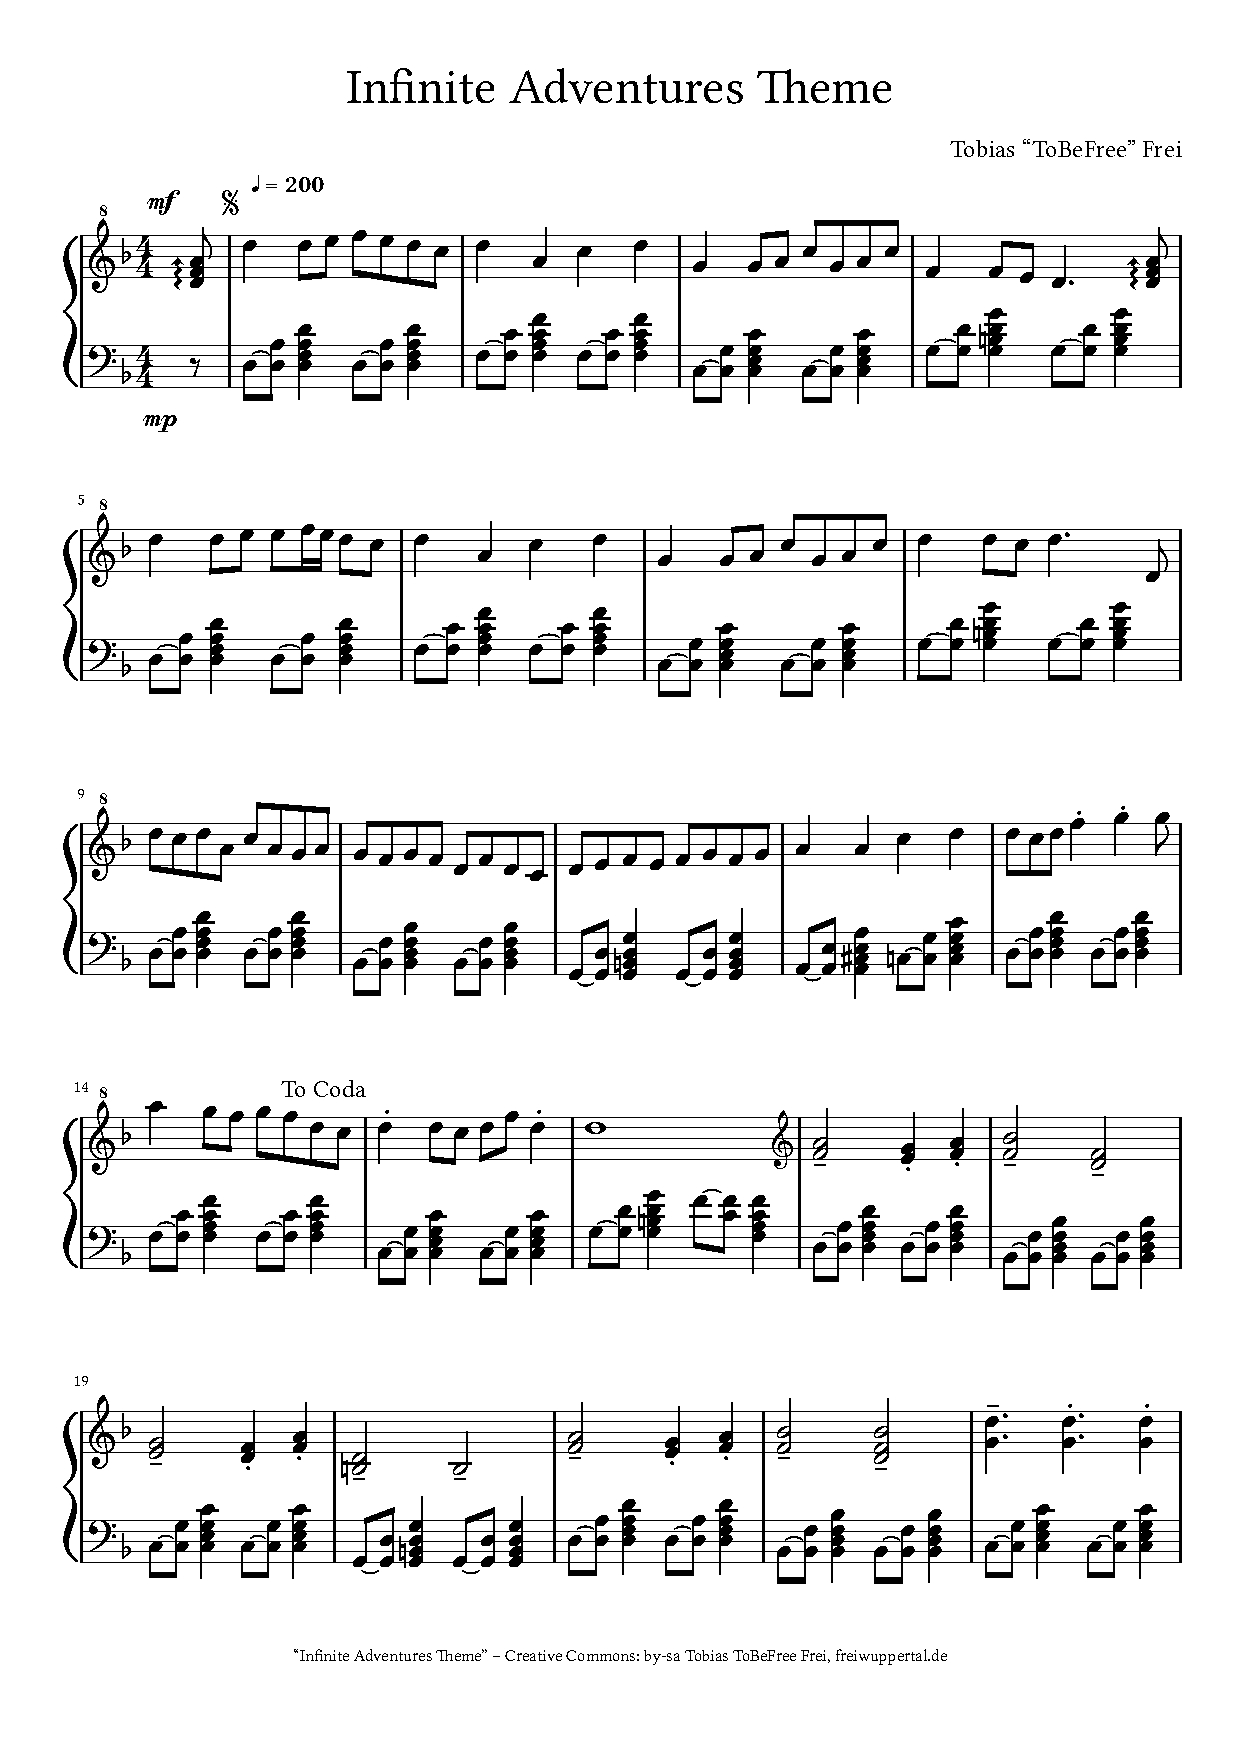
\includegraphics[width=\textwidth, page=1]{include-main-iatheme.pdf}
\end{figure}

\begin{figure}[p]
	\includegraphics[width=\textwidth, page=2]{include-main-iatheme.pdf}
\end{figure}


\chapter{Musikliste}

\textbf{Für Filmproduzenten, Träumer und Multitasking-Genies.}

\begin{itemize}
	\item Falls du ernsthaft einen Film zu diesem Buch drehen möchtest.
	\item Falls du das gesamte Buch bereits ausgelesen hast und die genannten Lieder vielleicht noch gar nicht kennst. Höre die Lieder und stelle dir dabei die Szenen vor. Wenn es schon keinen IA-Film gibt, kannst du wenigstens einen Film in deinem Kopf laufen lassen.
	\item Falls du beim Lesen Musik hören möchtest, die zur aktuellen Szene passt.
\end{itemize}

Diese Liste wurde von den Autoren zusammengestellt und impliziert keinerlei Unterstützung oder Befürwortung durch die Komponisten der Lieder.

Musik, die leider zum Veröffentlichungszeitpunkt nicht frei lizenziert war, ist durch \textit{kursiven Text} markiert. Eines Tages wird jedes dieser Lieder in die Gemeinfreiheit übergehen; der genaue Zeitpunkt hängt von verschiedenen Gesetzen ab.

Wir bieten auf infiniteadventures.de wahrscheinlich eine fertig nummerierte Musiksammlung der frei lizenzierten Lieder an, die einfach heruntergeladen und auf eine MP3-CD gebrannt werden kann. Für eine klassische Audio-CD ist die Gesamtlänge des Soundtracks deutlich zu groß.

Autoren der frei lizenzierten Musik:\\
Jason Shaw (Audionautix), audionautix.com\\
Marek »Wansti« Möckel, discarded-ideas.org\\
Nicolas Gasparini (Myuu), thedarkpiano.com\\
Tobias »ToBeFree« Frei, tfrei.de

\begin{enumerate}
    \item Titelmelodie:\\ »Infinite Adventures Theme« – Tobias »ToBeFree« Frei
    \item Orakel:\\ »Lazy Day« – Jason Shaw (Audionautix)
    \item Fluchtauto mit Automatikgetriebe:\\ »All Good In The Wood« – Jason Shaw (Audionautix)
    \item Kreuzfahrtschiff-Melodie (mehrfach verwendet):\\ »Bird In Hand« – Jason Shaw (Audionautix)
    \item Verrückte Zugfahrt:\\ »Code Blue« – Jason Shaw (Audionautix)
    \item Meister Orakel am Werk:\\ »Big Blues« – Jason Shaw (Audionautix)
    \item Flug nach Mallorca:\\ »Jennys Theme« – Jason Shaw (Audionautix)
    \item Die schwimmende Etage:\\ »Azitmuth« – Jason Shaw (Audionautix)
    \item Kreuzfahrt nach Manhattan:\\ »Bird In Hand« – Jason Shaw (Audionautix)
    \item Umrüstung des Helikopters:\\ »Boxcar Rag« – Jason Shaw (Audionautix)
    \item Mit dem Helikopter um die Welt:\\ »Latin House Bed« – Jason Shaw (Audionautix)
    \item Die Befreiung von Orakel in Südafrika:\\ »Boom« – Jason Shaw (Audionautix)
    \item Verfolgungsjagd über China:\\ »Checks For Free« – Jason Shaw (Audionautix)
    \item Mit dem Bus durch China:\\ »Busy Body« – Jason Shaw (Audionautix)
    \item Alexandra:\\ \textit{»Satoris Theme, Third Eye« aus Touhou 11 (Chireiden, Subterranean Animism) von Jun'ya Ota (ZUN)}
    \item Überfall auf Fort Knox:\\ »Line of Fire« – Jason Shaw (Audionautix)
    \item Flucht aus dem goldenen Gefängnis:\\ »Boogie Woogie Bed« – Jason Shaw (Audionautix)
    \item Einbruch beim FBI:\\ »Dark Mystery« – Jason Shaw (Audionautix)
    \item Flug nach Kanada, Teil 1:\\ \textit{»Wings of Death, Level 5« – Jochen Hippel (der Remix von Nils Schneider lohnt sich)}
    \item Flug nach Kanada, Teil 2:\\ »Med Tempo Rock« – Jason Shaw (Audionautix)
    \item Greater Sudbury:\\ »Landras Dream« – Jason Shaw (Audionautix)
    \item Am Lagerfeuer:\\ »Antarctica« – Jason Shaw (Audionautix)
    \item Flucht vom Lagerfeuer:\\ \textit{»Run Away« – Sunstroke Project, for Moldova at ESC 2010}
    \item Kanada nach USA, Teil 1:\\ \textit{»Wings of Death, Level 6« – Jochen Hippel (auch zu diesem Lied hat Nils Schneider einen tollen Remix erstellt)}
    \item Kanada nach USA, Teil 2:\\ \textit{Im Text wird ein Lied erwähnt. Einfach im richtigen Moment abspielen.}
    \item Sprung in die Tiefe:\\ »Funky Junky« – Jason Shaw (Audionautix)
    \item Bitte volltanken:\\ »Feel Good Rock« – Jason Shaw (Audionautix)
    \item Boeing 737 nach Deutschland:\\ \textit{»Like a Tiger« – Jayme Gutierrez (das Musikvideo ist gut)}
    \item Frees Theme:\\ \textit{»(Kenny the) Toffelskater« – Dubmood} 
    \item Aus der Ferne dringende Musik vom Filmfestival:\\ »Boots! Boots! Boots!« – Jason Shaw (Audionautix)
    \item Louvre-Mission:\\ »In Motion« – Jason Shaw (Audionautix)
    \item Flucht aus dem Louvre:\\ \textit{»Satono Nishida \& Mai Teireida, Crazy Backup Dancers« aus Touhou 16 (Tenkuushou, Hidden Star in Four Seasons) von Jun'ya Ota (ZUN)}
    \item Flug ins All:\\ \textit{»Major Tom« – Peter Schilling}
    \item Landung auf Örz:\\ Europahymne »Ode an die Freude«, ohne Text, letzter Satz der neunten Sinfonie in d-Moll op. 125 – Ludwig van Beethoven (gemeinfreie Version beispielsweise von der United States Navy Band)
    \item Dorf der Äöüzz:\\ »Forest Rhythm« – Jason Shaw (Audionautix)
    \item Örzkäpitöl:\\ »In The Field« – Jason Shaw (Audionautix)
    \item Betreten des Fööd-Geschäfts:\\ »Happy Little Elves« – Jason Shaw (Audionautix)
    \item Eigenes Haus:\\ »Keep It Real« – Jason Shaw (Audionautix)
    \item Reise der 4-6692 im Weltall:\\ \textit{»Journey of the Sorcerer« – Eagles}
    \item Nuklearer Winter:\\ »The Angels Weep« – Jason Shaw (Audionautix)    
    \item Weltraum-Hintergrundmusik, wenn keine andere läuft:\\ »Deep Space« – Jason Shaw (Audionautix)
    \item Anflug auf Cats Paw Sector OI-T c3-3:\\ »Go Not Gently« – Jason Shaw (Audionautix)
    \item Friedliche Welt: »Antarctica« – Jason Shaw (Audionautix)
    \item Landung im Gebirge:\\ »Intense Suspense« – Jason Shaw (Audionautix)
    \item Im Inneren der Möribünd Explörer:\\ »Dark Mystery« – Jason Shaw (Audionautix) 
    \item Ohne Licht durch die Höhle:\\ Mit leiser Lautstärke im Hintergrund:\\ »High Tension« – Jason Shaw (Audionautix)
    \item Alexandra im Einsatz:\\  \textit{»Sakuya Izayoi's Theme, Flowering Night« aus Touhou 10.5 (Hisouten, Scarlet Weather Rhapsody) von Jun'ya Ota (ZUN)}
    \item Flucht von Blärg:\\ \textit{»Star Fox (SNES), Corneria« – Hajime Hirasawa (der Remix von Qumu Music übertrifft das Original)}
    \item Sehenswürdigkeiten im Weltall:\\ »Leavin The Lights« – Jason Shaw (Audionautix)
    \item derair:\\ »House of Evil« – Jason Shaw (Audionautix)
    \item Raumgefecht:\\ »Fight Scene« – Jason Shaw (Audionautix)
    \item Rückkehr nach Örz:\\ »Chasin’ It« – Jason Shaw (Audionautix)
    \item Willkommen zurück:\\ »Shadow Of Truth« – Jason Shaw (Audionautix)
    \item Verurteilt:\\ »Legends Of The River« – Jason Shaw (Audionautix)
    \item Ankunft auf ugghy:\\ »Event Horizon« – Jason Shaw (Audionautix)
    \item Ausbruch:\\ »Intro Action« – Jason Shaw (Audionautix)
    \item Floating Island sucht Material:\\ »Energy Bed 2« – Jason Shaw (Audionautix)
    \item Im Inneren des uggy-Raumschiffs auf Örs-Anflug:\\ »Harsh Alien Machine« – Jason Shaw (Audionautix)
    \item Angriff der uggy-Zerstörungsflotte:\\ »Long Live Death« – Jason Shaw (Audionautix)
    \item SoulOfTheInternet:\\ \textit{»Thraddash: Culture 19« (Remix des Liedes »Thraddash Theme« aus Star Control II, 1992, von Riku Nuottajärvi) – Espen Gätzschmann und Tore Aune Fjellstad}
    \item SOTIs Welt:\\ »Ohm« von Audionautix
    \item Landung der Protagonisten auf der Erde:\\ »Lexicon« – Jason Shaw (Audionautix)
    \item Das Haus, in dem noch alles normal ist:\\ »Paper Wings« von Audionautix
    \item Überraschung im BIDWA:\\ »Peppers Funk« – Jason Shaw (Audionautix)
    \item Vorbereitung:\\ »Doghouse« – Jason Shaw (Audionautix)
    \item Credits am Ende:\\ \textit{»Cydonian Sky« – Dubmood (Kalle Jonsson)}
    \item \textbf{Geplant für die Infinite Adventures 2:}\\ Titelmelodie:\\ Infinite Adventures Theme 2\\(Titelmelodie-Platzhalter:\\ »Sleigh Ride« – Tobias »ToBeFree« Frei)
    \item Lkw zum Pentagon:\\ »Piledriver« – Jason Shaw (Audionautix) 
    \item In den Gängen des Pentagon:\\ »Alien Sunset« – Jason Shaw (Audionautix)
    \item Das leere Büro:\\ »Kicked up Pumps« – Jason Shaw (Audionautix)
    \item Eiswüste Antarktis:\\ »Plantation« – Jason Shaw (Audionautix)
    \item Im Zentrum der Macht:\\ »Megaton Drop« – Jason Shaw (Audionautix)
    \item Erfolg:\\ »Intro 5« – Jason Shaw (Audionautix)
    \item Erde befreit:\\ »Away In A Manger Edm« – Jason Shaw (Audionautix)
    \item \textbf{Generelle Vorschläge für Zeit-Vergeht-Szenen:}\\ »Forest Theme for Piano and Recorder« – Marek »Wansti« Möckel
    \item »Forest Dance« – Marek »Wansti« Möckel
    \item »Rabbit Holes« – Marek »Wansti« Möckel
    \item »Riding The Wind« – Marek »Wansti« Möckel
    \item »Nightfall« – Marek »Wansti« Möckel
    \item »Phase Shifter« – Jason Shaw (Audionautix)
    \item »Opus One« – Jason Shaw (Audionautix)
    \item »Pop Rock Bed« – Jason Shaw (Audionautix)
    \item »Over Time« – Jason Shaw (Audionautix)
    \item »Time Passing By« – Jason Shaw (Audionautix)
    \item »The Voyage« – Jason Shaw (Audionautix)
    \item »Triangle« – Jason Shaw (Audionautix)
    \item »In A World« – Jason Shaw (Audionautix)
    \item »Quiet« – Jason Shaw (Audionautix)
    \item »Renaissance« – Jason Shaw (Audionautix)
    \item »River Meditation« – Jason Shaw (Audionautix)
    \item »Serious Drama« – Jason Shaw (Audionautix)
    \item »Serious Piano« – Jason Shaw (Audionautix)
    \item »Evil Returns«– Nicolas Gasparini (Myuu)
    \item »Moonlight Menschen« – Nicolas Gasparini (Myuu)
    \item \textit{»Extra Stage Theme, Last Remote« aus Touhou 11 (Chireiden, Subterranean Animism) von Jun'ya Ota (ZUN)}
    \item \textit{»Hong Meiling's Theme, Shanghai Teahouse / Chinese Tea« aus Touhou 12.3 (Hisoutensoku, Unthinkable Natural Law) von Jun'ya Ota (ZUN)}
    \item \textit{»Reimu Hakurei's Theme, Dichromatic Lotus Butterfly / Ancients« aus Touhou 12.3 (Hisoutensoku, Unthinkable Natural Law) von Jun'ya Ota (ZUN)}
    \item \textit{»Reimu Hakurei's Theme, Dichromatic Lotus Butterfly / Red and White« aus Touhou 14.5 (Shinpiroku, Urban Legend in Limbo) von Jun'ya Ota (ZUN) und Comp von Butaotome}
    \item \textit{»Sweet Dreams« – Elwood}
    \item \textbf{Generelle Vorschläge für Action-Szenen:}\\ »Prophecy« – Marek »Wansti« Möckel
    \item »Fortress« – Marek »Wansti« Möckel
    \item »Ectoplasm« – Jason Shaw (Audionautix)
    \item »Delusion 32« – Jason Shaw (Audionautix)
    \item »Pop Metal« – Jason Shaw (Audionautix)
    \item »Bustin Loose« / »Bustin Loose W Lead« – Jason Shaw (Audionautix)
    \item »Pentagram« – Jason Shaw (Audionautix)
    \item »Periscope« – Jason Shaw (Audionautix)
    \item »Sports Action« – Jason Shaw (Audionautix)
    \item »Pyramids« – Jason Shaw (Audionautix)    
    \item »Night Runner« – Jason Shaw (Audionautix)
    \item \textit{»Cirno's Theme, Otenba Koi Musume / Tomboyish Girl in Love« aus Touhou 12.3 (Hisoutensoku, Unthinkable Natural Law) von Jun'ya Ota (ZUN)}
    \item \textit{»Eirin Yagokoro's Theme, Gensokyo Millenium / History of the Moon« aus Touhou 08 (Eiyashou, Imperishable Night) von Jun'ya Ota (ZUN)}
    \item \textit{»Fujiwara no Mokou's Theme, Reach for the Moon, Immortal Smoke« aus Touhou 08 (Eiyashou, Imperishable Night) von Jun'ya Ota (ZUN)}
    \item \textit{»Irresistible« – Fall Out Boy}
    \item \textit{»Immortals«  – Fall Out Boy}
    \item \textit{»Megalovania« (aus Undertale von Toby Fox)}

\end{enumerate}




\chapter{Orakels Zeichnungen}

Als das Freiwuppertal-Forum noch aktiv genutzt wurde, hat Orakel einige Zeichnungen erstellt, in denen die Forenbenutzer satirisch dargestellt wurden. Da die Protagonisten der Infinite Adventures ihre Namen von den Benutzern dieses Forums erhalten haben, sind gewisse Überschneidungen mit dem Inhalt des Romans erkennbar. Die Zeichnungen wurden \textit{nicht} für die Infinite Adventures erstellt, dürfen aber als ergänzendes Bonusmaterial nicht fehlen.

Wir werden voraussichtlich einen DIN-A4-Bonusband zu den Infinite Adventures veröffentlichen. Eine Ringbindung soll leichtes Umblättern und Herausnehmen des Bonusmaterials ermöglichen. In diesem Bonusband werden weitere Zeichnungen enthalten sein.

\begin{figure}[p]
	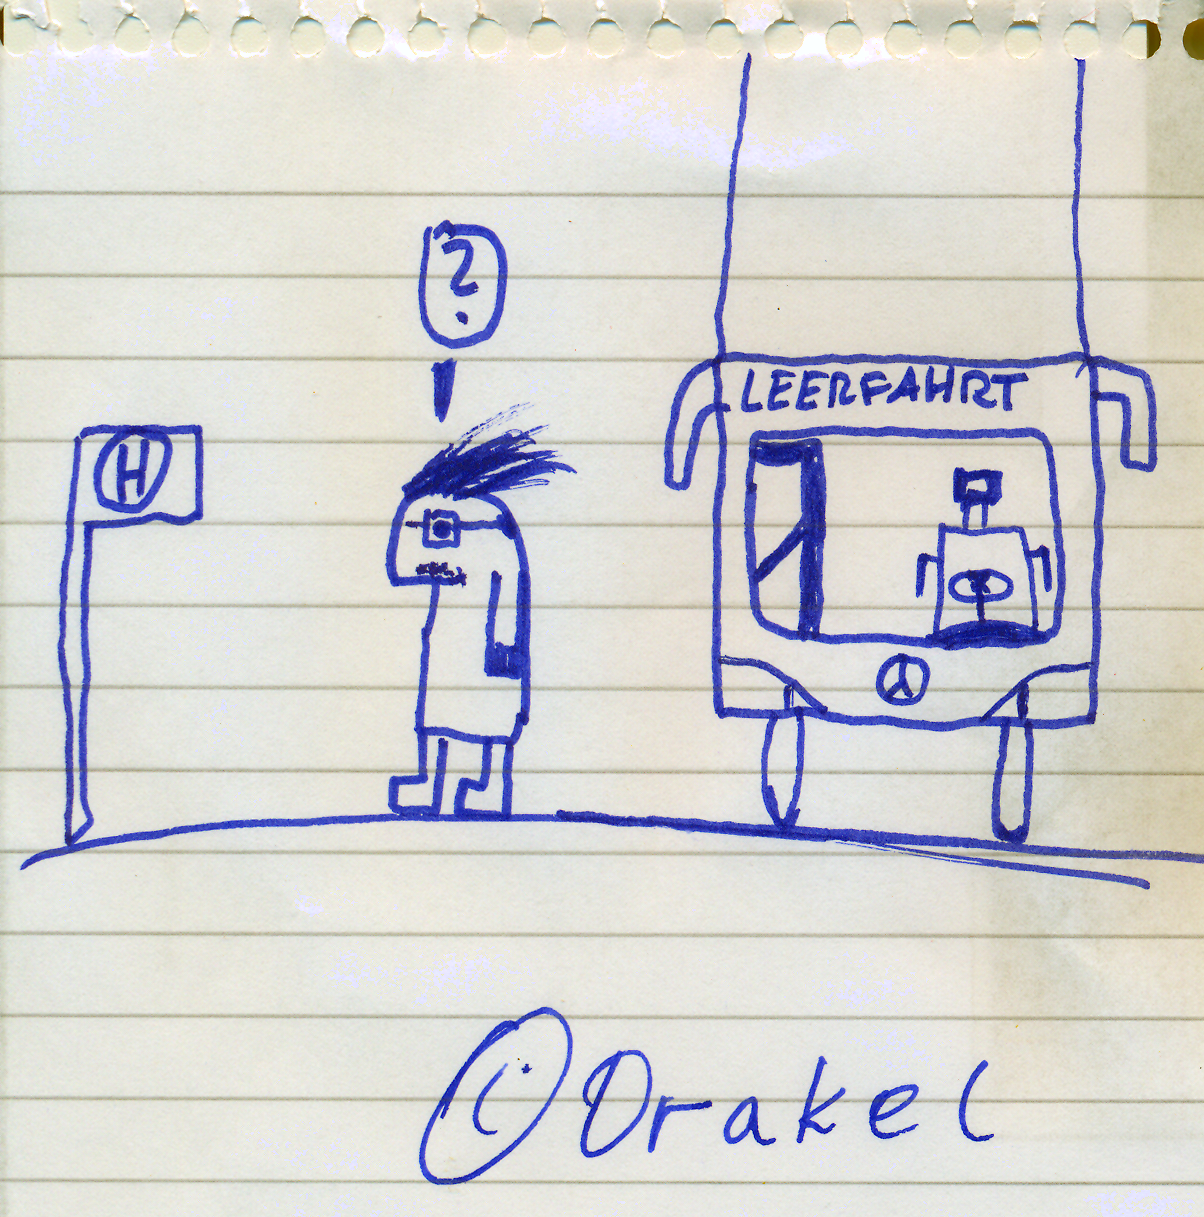
\includegraphics[width=\linewidth]{include-main-orakel-leerfahrt.png}
	\caption{„Leerfahrt“. CC by-sa 4.0: Mirco Hensel}
\end{figure}

\begin{figure}[p]
	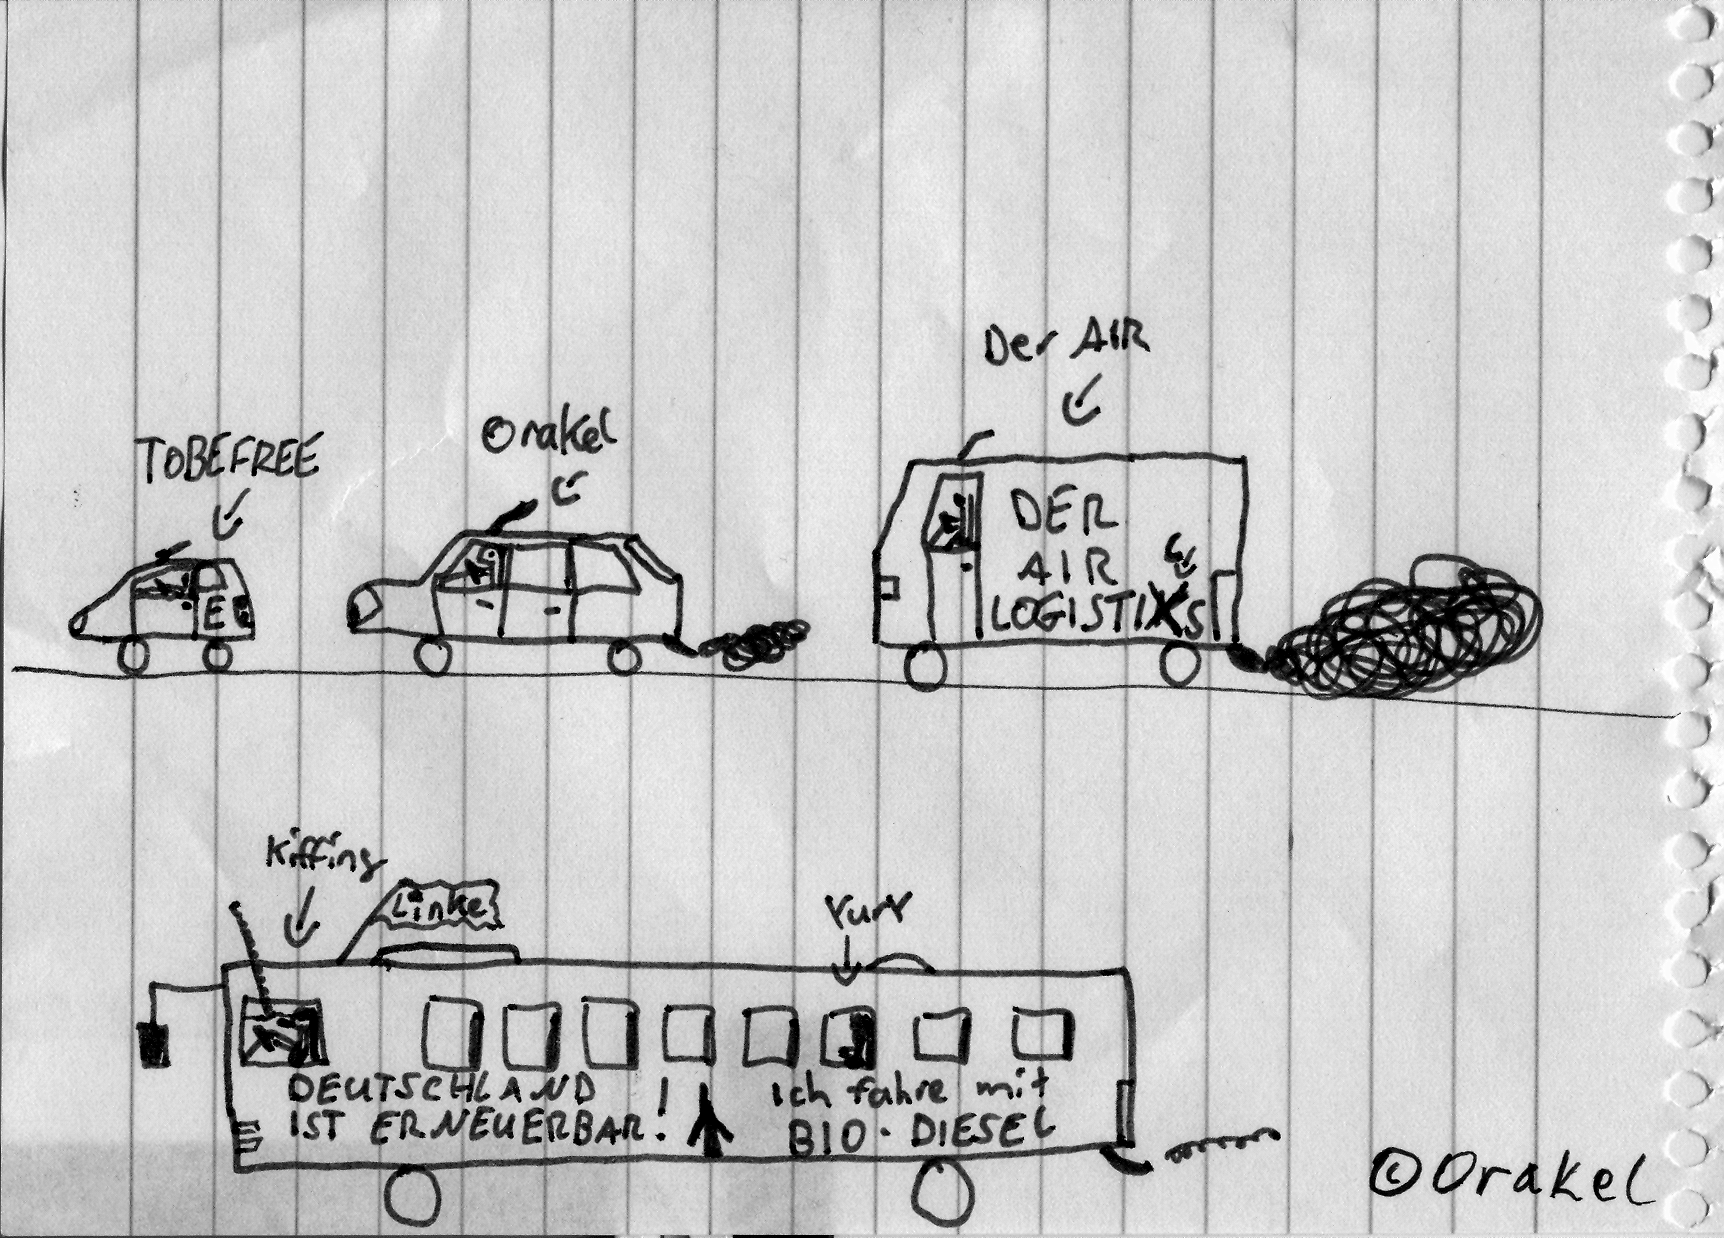
\includegraphics[width=\linewidth]{include-main-orakel-motion.png}
	\caption{„Motion“. CC by-sa 4.0: Mirco Hensel}
\end{figure}


\chapter{Karte der Galaxis}

Auch diese Karte wird in größerem Format zu einem Teil des Bonusbands werden.

\begin{figure}[p]
	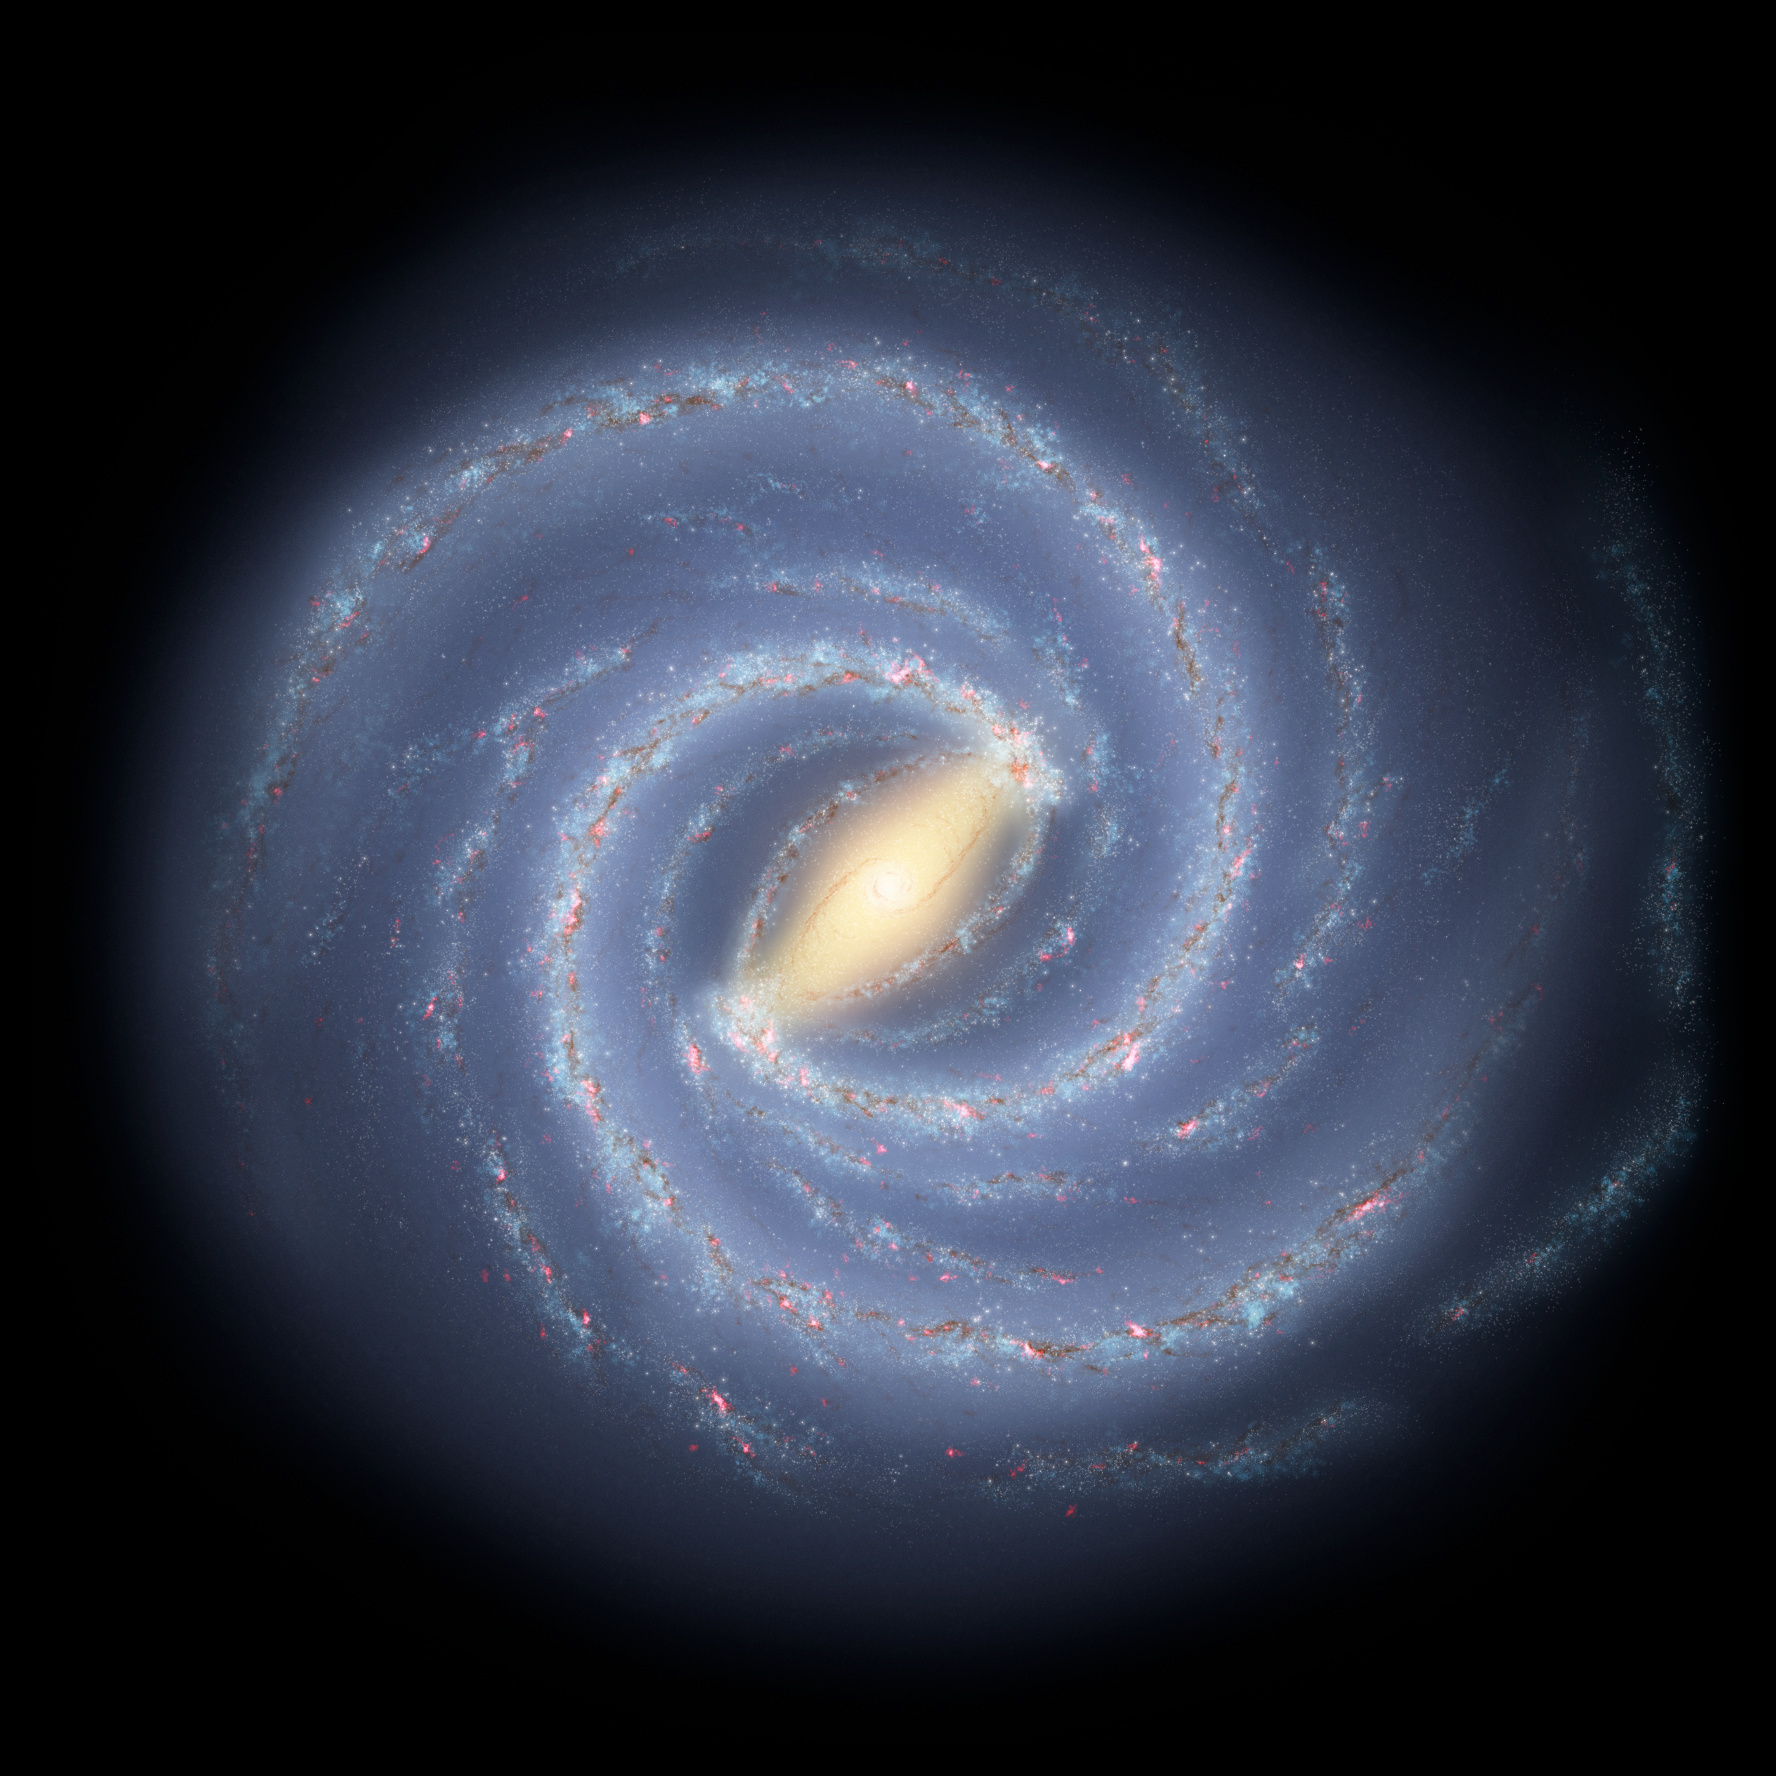
\includegraphics[width=\linewidth]{include-main-galaxymap-square-bg.jpg}
	\caption{Unsere Milchstraße}
\end{figure}

\begin{figure}[p]
	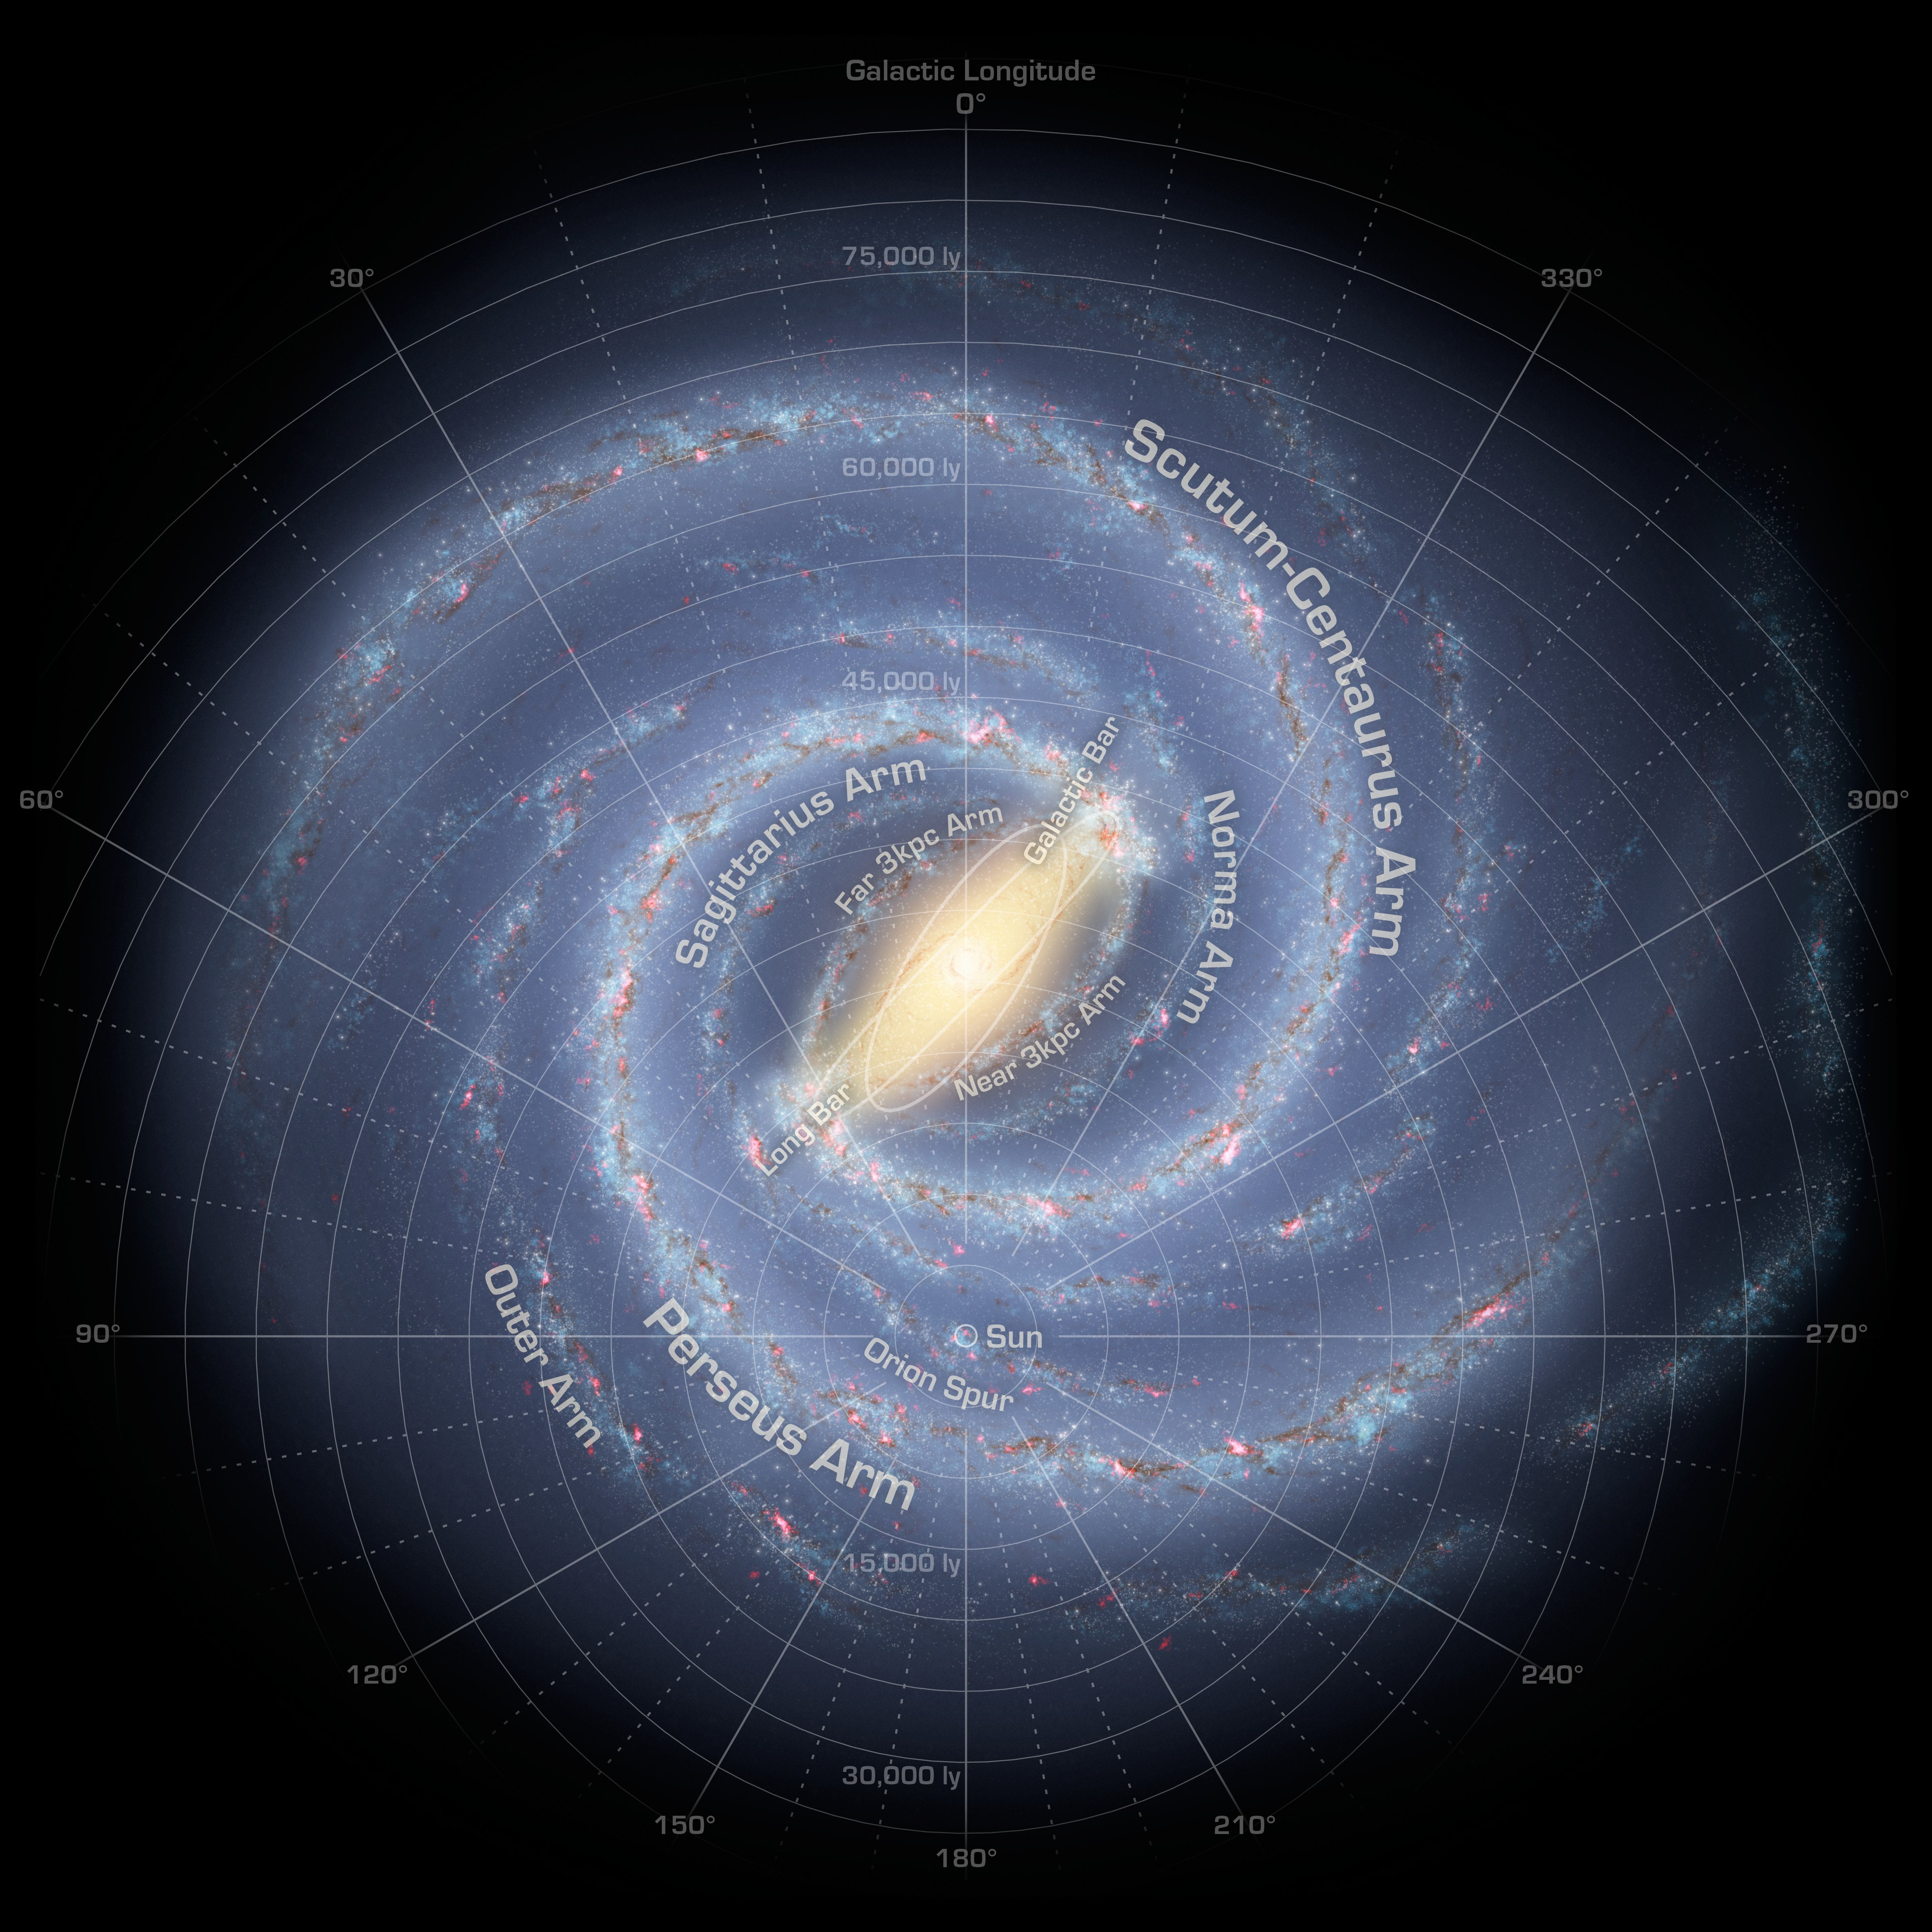
\includegraphics[width=\linewidth]{include-main-galaxymap-square.jpg}
	\caption{Galaktisches Koordinatensystem}
\end{figure}


\chapter{Helden von Örz}


\chapter{Auszug: Original-Forenthread}

So sind die Infinite Adventures entstanden: Orakel, yury und Free haben Beiträge in einem Internetforum geschrieben. In diesem Auszug sieht man, wie innerhalb von vier Stunden alle drei Autoren einen Teil zum Roman beigetragen haben. Außerdem ist dies der Beweis dafür, dass wir bereits im September 2010 das Aufkommen von Quantencomputern und DNA-Festplatten vorhergesagt haben.

Orakels Beitrag enthält ein Handygespräch, das damals noch über mehrere Galaxien hinweg geführt wurde. Auch in der heutigen Fassung mit einer Distanz von über 4000 Lichtjahren zur Erde verfehlt der Anruf seine überraschende Wirkung nicht.

Auf die Idee, man könnte die aus Fort Knox gestohlenen Goldbarren auf Örz verkaufen, waren wir damals noch nicht gekommen. Daher muss Free für den Quantencomputer einen Kredit aufnehmen. Dass schwere körperliche Arbeit auf dem fortschrittlichen Planeten nicht von Robotern erledigt wurde, wirkt im Nachhinein merkwürdig.

yury überraschte uns dann mit einer Verhaftung aus heiterem Himmel. Sein Kommentar dazu: »Ich hab schon einen Hintergedanken, aber der Plan ist doch, dass ihr jetzt was völlig anderes, für mich unerwartetes schreibt und die IA dadurch interessant wird… also lasst euch was einfallen! ;)«

Das Design des Forums hat sich irgendwann durch ein Update geändert; dieses aktuelle Bildschirmfoto zeigt nicht das ursprüngliche Aussehen des Forums. Zudem fällt auf, dass die Geschichte damals einen anderen Titel hatte, und dass Free anders hieß.

\begin{figure}[p]
	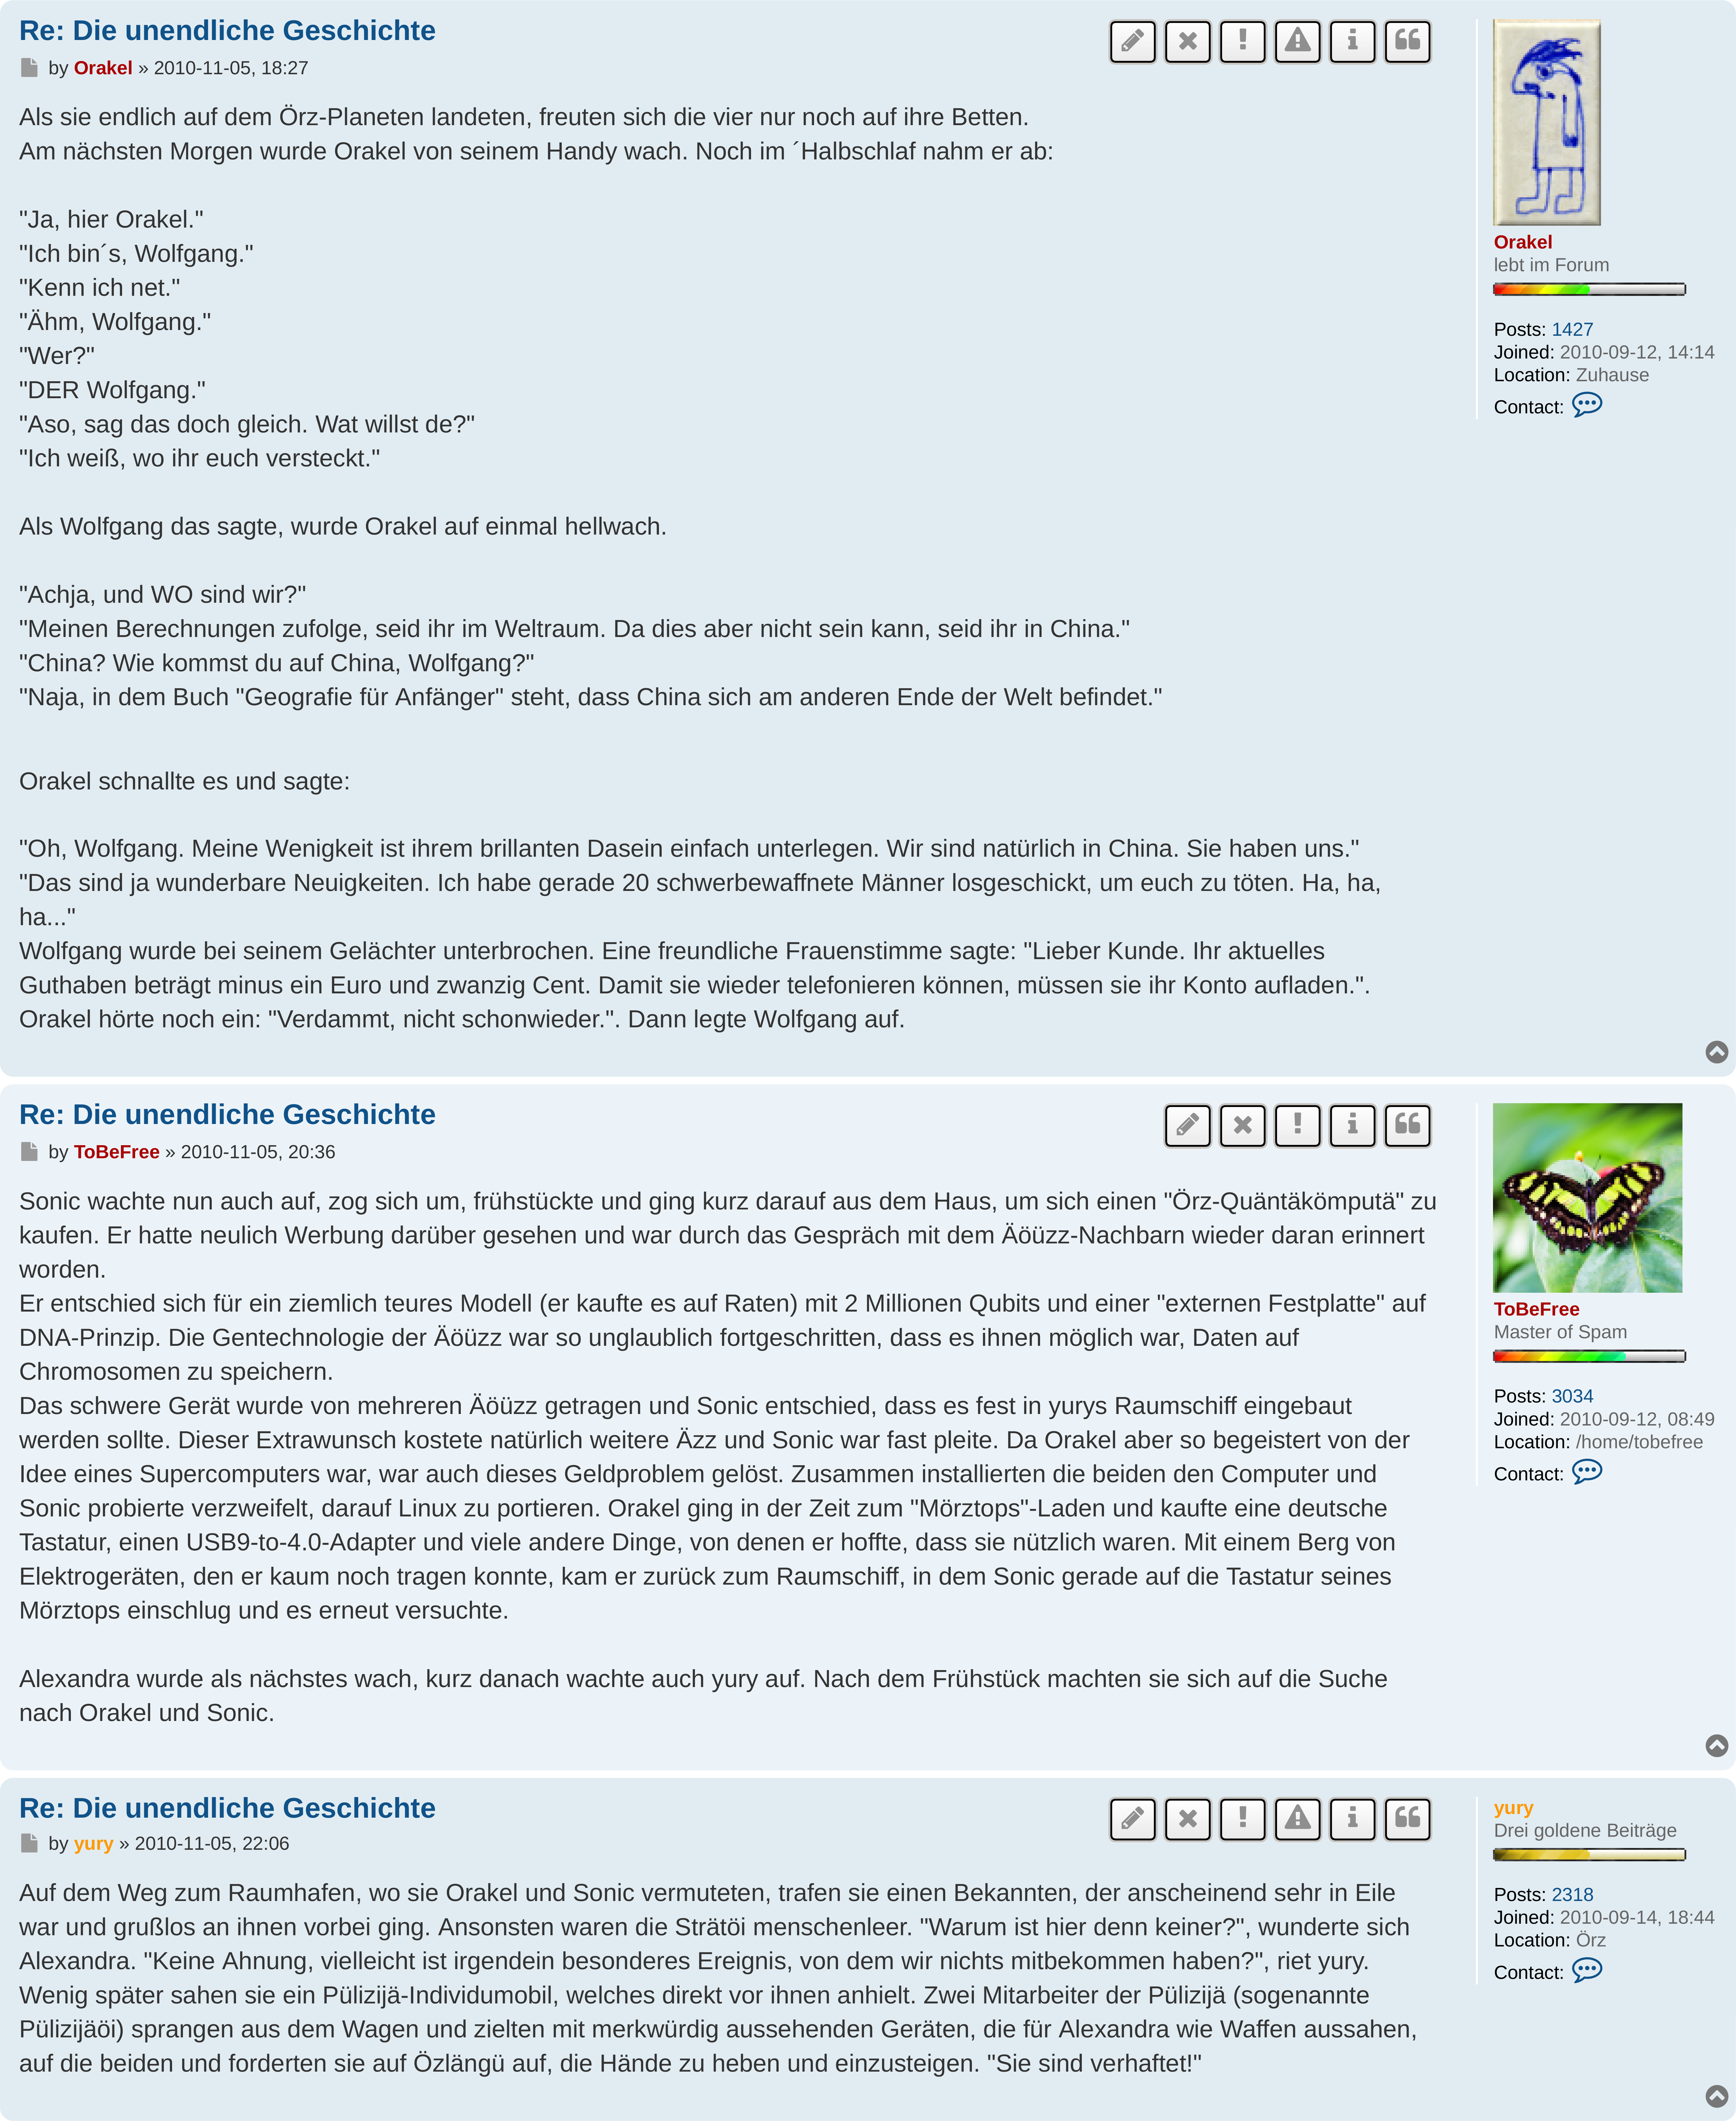
\includegraphics[width=\linewidth]{include-main-iathread-original-dna.png}
	\caption{https://freiwuppertal.de/forum\#: Interner Schreibbereich}
\end{figure}


\chapter{Bildquellen}

Alle verwendeten Bilder sind frei lizenziert. Die Verwendung der Bilder in diesem Roman impliziert keinerlei Unterstützung oder Befürwortung durch ihre Schöpfer.

\begin{itemize}
	\item \textbf{Buchcover:} CC0-Lizenz / Public Domain.\\ Yuri\_B, pixabay.com
	\item \textbf{Teil-2-Titelbild:} CC0-Lizenz / Public Domain.\\ Leandro Barco (Wortley, pixabay.com)
	\item \textbf{Galaktische Karte:} Public Domain.\\ NASA/JPL-Caltech/R. Hurt (SSC/Caltech).\\ https://commons.wikimedia.org/wiki/\\File:236084main\_MilkyWay-full-annotated.jpg
	\item \textbf{NGC 6188/6193 und NGC 6334:} Public Domain.\\ Dylan O'Donnell, deography.com\\ »That means it’s free for you to use, now and forever. You don’t even have to credit me for it. […] Photography is not my job and I’d rather not kill any enthusiasm I have for it by accepting money for the obligation to take photos.

So use them, by all means. You don’t have to credit me if you don’t want to, but I love seeing my work out there in the wild being used, mixed and remixed. Send me a link, I’d love to see what you do!« (https://deography.com/yes-its-free/\#, Abruf 2018-01-01)
	\item \textbf{Helixnebel (NGC 7293):} Public Domain.\\ NASA/JPL-Caltech.\\https://commons.wikimedia.org/wiki/\\File:Helix\_Nebula\_-\_Unraveling\_at\_the\_Seams.jpg
	\item \textbf{Orakels Zeichnungen und Orakels Avatar:}\\ Creative Commons by-sa 4.0.\\ Mirco Hensel\\Eine Kopie der Lizenz befindet sich am Ende des Buches.
	\item \textbf{ToBeFrees Avatar:}\\ CC0-Lizenz / Public Domain.\\ jill111, pixabay.com
\end{itemize}

Bei den Bildern in diesem Roman handelt es sich nicht um die exakten Originalbilder, sondern um Abwandlungen (Weißabgleich, Helligkeit, Kontrast, Sättigung, Schärfung, Zuschnitt etc.) erstellt durch Tobias Frei.

Für die Infinite Adventures erstellte Abwandlungen frei lizenzierter Werke wurden auf Wikimedia Commons hochgeladen und auf diese Weise an die Gemeinschaft zurückgegeben.

Yuri\_B, Leandro Barco und Dylan O'Donnell erhalten jeweils mindestens ein kostenloses Exemplar des Buches. Zum Dank für die frei nutzbaren Bilder wird persönliches Bonusmaterial erstellt.


\chapter{Lizenz des Buchinhalts}

\textbf{Infinite Adventures (c) by\\ Mirco Hensel, yury, Tobias Frei, infiniteadventures.de}

Falls du die Rechte in dieser Lizenz nutzen möchtest, musst du sie vollständig gelesen und verstanden haben. Es genügt nicht, nur die »menschenlesbare Zusammenfassung« zu lesen. Aus diesem Grund bieten wir keine solche Zusammenfassung an.

This novel is licensed under a
Creative Commons Attribution-ShareAlike 4.0 International License.

You should have received a copy of the license along with this
work. If not, see https://creativecommons.org/licenses/by-sa/4.0/legalcode

You are required to actually read and understand the full text of the license, not just the »human-readable summary«.

Attribution-ShareAlike 4.0 International

======

Creative Commons Corporation ("Creative Commons") is not a law firm and
does not provide legal services or legal advice. Distribution of
Creative Commons public licenses does not create a lawyer-client or
other relationship. Creative Commons makes its licenses and related
information available on an "as-is" basis. Creative Commons gives no
warranties regarding its licenses, any material licensed under their
terms and conditions, or any related information. Creative Commons
disclaims all liability for damages resulting from their use to the
fullest extent possible.

Using Creative Commons Public Licenses

Creative Commons public licenses provide a standard set of terms and
conditions that creators and other rights holders may use to share
original works of authorship and other material subject to copyright
and certain other rights specified in the public license below. The
following considerations are for informational purposes only, are not
exhaustive, and do not form part of our licenses.

     Considerations for licensors: Our public licenses are
     intended for use by those authorized to give the public
     permission to use material in ways otherwise restricted by
     copyright and certain other rights. Our licenses are
     irrevocable. Licensors should read and understand the terms
     and conditions of the license they choose before applying it.
     Licensors should also secure all rights necessary before
     applying our licenses so that the public can reuse the
     material as expected. Licensors should clearly mark any
     material not subject to the license. This includes other CC-
     licensed material, or material used under an exception or
     limitation to copyright. More considerations for licensors:
	wiki.creativecommons.org/Considerations\_for\_licensors

     Considerations for the public: By using one of our public
     licenses, a licensor grants the public permission to use the
     licensed material under specified terms and conditions. If
     the licensor's permission is not necessary for any reason--for
     example, because of any applicable exception or limitation to
     copyright--then that use is not regulated by the license. Our
     licenses grant only permissions under copyright and certain
     other rights that a licensor has authority to grant. Use of
     the licensed material may still be restricted for other
     reasons, including because others have copyright or other
     rights in the material. A licensor may make special requests,
     such as asking that all changes be marked or described.
     Although not required by our licenses, you are encouraged to
     respect those requests where reasonable. More considerations
     for the public: 
	wiki.creativecommons.org/Considerations\_for\_licensees

=====

Creative Commons Attribution-ShareAlike 4.0 International Public
License

By exercising the Licensed Rights (defined below), You accept and agree
to be bound by the terms and conditions of this Creative Commons
Attribution-ShareAlike 4.0 International Public License ("Public
License"). To the extent this Public License may be interpreted as a
contract, You are granted the Licensed Rights in consideration of Your
acceptance of these terms and conditions, and the Licensor grants You
such rights in consideration of benefits the Licensor receives from
making the Licensed Material available under these terms and
conditions.


Section 1 -- Definitions.

  a. Adapted Material means material subject to Copyright and Similar
     Rights that is derived from or based upon the Licensed Material
     and in which the Licensed Material is translated, altered,
     arranged, transformed, or otherwise modified in a manner requiring
     permission under the Copyright and Similar Rights held by the
     Licensor. For purposes of this Public License, where the Licensed
     Material is a musical work, performance, or sound recording,
     Adapted Material is always produced where the Licensed Material is
     synched in timed relation with a moving image.

  b. Adapter's License means the license You apply to Your Copyright
     and Similar Rights in Your contributions to Adapted Material in
     accordance with the terms and conditions of this Public License.

  c. BY-SA Compatible License means a license listed at
     creativecommons.org/compatiblelicenses, approved by Creative
     Commons as essentially the equivalent of this Public License.

  d. Copyright and Similar Rights means copyright and/or similar rights
     closely related to copyright including, without limitation,
     performance, broadcast, sound recording, and Sui Generis Database
     Rights, without regard to how the rights are labeled or
     categorized. For purposes of this Public License, the rights
     specified in Section 2(b)(1)-(2) are not Copyright and Similar
     Rights.

  e. Effective Technological Measures means those measures that, in the
     absence of proper authority, may not be circumvented under laws
     fulfilling obligations under Article 11 of the WIPO Copyright
     Treaty adopted on December 20, 1996, and/or similar international
     agreements.

  f. Exceptions and Limitations means fair use, fair dealing, and/or
     any other exception or limitation to Copyright and Similar Rights
     that applies to Your use of the Licensed Material.

  g. License Elements means the license attributes listed in the name
     of a Creative Commons Public License. The License Elements of this
     Public License are Attribution and ShareAlike.

  h. Licensed Material means the artistic or literary work, database,
     or other material to which the Licensor applied this Public
     License.

  i. Licensed Rights means the rights granted to You subject to the
     terms and conditions of this Public License, which are limited to
     all Copyright and Similar Rights that apply to Your use of the
     Licensed Material and that the Licensor has authority to license.

  j. Licensor means the individual(s) or entity(ies) granting rights
     under this Public License.

  k. Share means to provide material to the public by any means or
     process that requires permission under the Licensed Rights, such
     as reproduction, public display, public performance, distribution,
     dissemination, communication, or importation, and to make material
     available to the public including in ways that members of the
     public may access the material from a place and at a time
     individually chosen by them.

  l. Sui Generis Database Rights means rights other than copyright
     resulting from Directive 96/9/EC of the European Parliament and of
     the Council of 11 March 1996 on the legal protection of databases,
     as amended and/or succeeded, as well as other essentially
     equivalent rights anywhere in the world.

  m. You means the individual or entity exercising the Licensed Rights
     under this Public License. Your has a corresponding meaning.


Section 2 -- Scope.

  a. License grant.

       1. Subject to the terms and conditions of this Public License,
          the Licensor hereby grants You a worldwide, royalty-free,
          non-sublicensable, non-exclusive, irrevocable license to
          exercise the Licensed Rights in the Licensed Material to:

            a. reproduce and Share the Licensed Material, in whole or
               in part; and

            b. produce, reproduce, and Share Adapted Material.

       2. Exceptions and Limitations. For the avoidance of doubt, where
          Exceptions and Limitations apply to Your use, this Public
          License does not apply, and You do not need to comply with
          its terms and conditions.

       3. Term. The term of this Public License is specified in Section
          6(a).

       4. Media and formats; technical modifications allowed. The
          Licensor authorizes You to exercise the Licensed Rights in
          all media and formats whether now known or hereafter created,
          and to make technical modifications necessary to do so. The
          Licensor waives and/or agrees not to assert any right or
          authority to forbid You from making technical modifications
          necessary to exercise the Licensed Rights, including
          technical modifications necessary to circumvent Effective
          Technological Measures. For purposes of this Public License,
          simply making modifications authorized by this Section 2(a)
          (4) never produces Adapted Material.

       5. Downstream recipients.

            a. Offer from the Licensor -- Licensed Material. Every
               recipient of the Licensed Material automatically
               receives an offer from the Licensor to exercise the
               Licensed Rights under the terms and conditions of this
               Public License.

            b. Additional offer from the Licensor -- Adapted Material.
               Every recipient of Adapted Material from You
               automatically receives an offer from the Licensor to
               exercise the Licensed Rights in the Adapted Material
               under the conditions of the Adapter's License You apply.

            c. No downstream restrictions. You may not offer or impose
               any additional or different terms or conditions on, or
               apply any Effective Technological Measures to, the
               Licensed Material if doing so restricts exercise of the
               Licensed Rights by any recipient of the Licensed
               Material.

       6. No endorsement. Nothing in this Public License constitutes or
          may be construed as permission to assert or imply that You
          are, or that Your use of the Licensed Material is, connected
          with, or sponsored, endorsed, or granted official status by,
          the Licensor or others designated to receive attribution as
          provided in Section 3(a)(1)(A)(i).

  b. Other rights.

       1. Moral rights, such as the right of integrity, are not
          licensed under this Public License, nor are publicity,
          privacy, and/or other similar personality rights; however, to
          the extent possible, the Licensor waives and/or agrees not to
          assert any such rights held by the Licensor to the limited
          extent necessary to allow You to exercise the Licensed
          Rights, but not otherwise.

       2. Patent and trademark rights are not licensed under this
          Public License.

       3. To the extent possible, the Licensor waives any right to
          collect royalties from You for the exercise of the Licensed
          Rights, whether directly or through a collecting society
          under any voluntary or waivable statutory or compulsory
          licensing scheme. In all other cases the Licensor expressly
          reserves any right to collect such royalties.


Section 3 -- License Conditions.

Your exercise of the Licensed Rights is expressly made subject to the
following conditions.

  a. Attribution.

       1. If You Share the Licensed Material (including in modified
          form), You must:

            a. retain the following if it is supplied by the Licensor
               with the Licensed Material:

                 i. identification of the creator(s) of the Licensed
                    Material and any others designated to receive
                    attribution, in any reasonable manner requested by
                    the Licensor (including by pseudonym if
                    designated);

                ii. a copyright notice;

               iii. a notice that refers to this Public License;

                iv. a notice that refers to the disclaimer of
                    warranties;

                 v. a URI or hyperlink to the Licensed Material to the
                    extent reasonably practicable;

            b. indicate if You modified the Licensed Material and
               retain an indication of any previous modifications; and

            c. indicate the Licensed Material is licensed under this
               Public License, and include the text of, or the URI or
               hyperlink to, this Public License.

       2. You may satisfy the conditions in Section 3(a)(1) in any
          reasonable manner based on the medium, means, and context in
          which You Share the Licensed Material. For example, it may be
          reasonable to satisfy the conditions by providing a URI or
          hyperlink to a resource that includes the required
          information.

       3. If requested by the Licensor, You must remove any of the
          information required by Section 3(a)(1)(A) to the extent
          reasonably practicable.

  b. ShareAlike.

     In addition to the conditions in Section 3(a), if You Share
     Adapted Material You produce, the following conditions also apply.

       1. The Adapter's License You apply must be a Creative Commons
          license with the same License Elements, this version or
          later, or a BY-SA Compatible License.

       2. You must include the text of, or the URI or hyperlink to, the
          Adapter's License You apply. You may satisfy this condition
          in any reasonable manner based on the medium, means, and
          context in which You Share Adapted Material.

       3. You may not offer or impose any additional or different terms
          or conditions on, or apply any Effective Technological
          Measures to, Adapted Material that restrict exercise of the
          rights granted under the Adapter's License You apply.


Section 4 -- Sui Generis Database Rights.

Where the Licensed Rights include Sui Generis Database Rights that
apply to Your use of the Licensed Material:

  a. for the avoidance of doubt, Section 2(a)(1) grants You the right
     to extract, reuse, reproduce, and Share all or a substantial
     portion of the contents of the database;

  b. if You include all or a substantial portion of the database
     contents in a database in which You have Sui Generis Database
     Rights, then the database in which You have Sui Generis Database
     Rights (but not its individual contents) is Adapted Material,

     including for purposes of Section 3(b); and
  c. You must comply with the conditions in Section 3(a) if You Share
     all or a substantial portion of the contents of the database.

For the avoidance of doubt, this Section 4 supplements and does not
replace Your obligations under this Public License where the Licensed
Rights include other Copyright and Similar Rights.


Section 5 -- Disclaimer of Warranties and Limitation of Liability.

  a. UNLESS OTHERWISE SEPARATELY UNDERTAKEN BY THE LICENSOR, TO THE
     EXTENT POSSIBLE, THE LICENSOR OFFERS THE LICENSED MATERIAL AS-IS
     AND AS-AVAILABLE, AND MAKES NO REPRESENTATIONS OR WARRANTIES OF
     ANY KIND CONCERNING THE LICENSED MATERIAL, WHETHER EXPRESS,
     IMPLIED, STATUTORY, OR OTHER. THIS INCLUDES, WITHOUT LIMITATION,
     WARRANTIES OF TITLE, MERCHANTABILITY, FITNESS FOR A PARTICULAR
     PURPOSE, NON-INFRINGEMENT, ABSENCE OF LATENT OR OTHER DEFECTS,
     ACCURACY, OR THE PRESENCE OR ABSENCE OF ERRORS, WHETHER OR NOT
     KNOWN OR DISCOVERABLE. WHERE DISCLAIMERS OF WARRANTIES ARE NOT
     ALLOWED IN FULL OR IN PART, THIS DISCLAIMER MAY NOT APPLY TO YOU.

  b. TO THE EXTENT POSSIBLE, IN NO EVENT WILL THE LICENSOR BE LIABLE
     TO YOU ON ANY LEGAL THEORY (INCLUDING, WITHOUT LIMITATION,
     NEGLIGENCE) OR OTHERWISE FOR ANY DIRECT, SPECIAL, INDIRECT,
     INCIDENTAL, CONSEQUENTIAL, PUNITIVE, EXEMPLARY, OR OTHER LOSSES,
     COSTS, EXPENSES, OR DAMAGES ARISING OUT OF THIS PUBLIC LICENSE OR
     USE OF THE LICENSED MATERIAL, EVEN IF THE LICENSOR HAS BEEN
     ADVISED OF THE POSSIBILITY OF SUCH LOSSES, COSTS, EXPENSES, OR
     DAMAGES. WHERE A LIMITATION OF LIABILITY IS NOT ALLOWED IN FULL OR
     IN PART, THIS LIMITATION MAY NOT APPLY TO YOU.

  c. The disclaimer of warranties and limitation of liability provided
     above shall be interpreted in a manner that, to the extent
     possible, most closely approximates an absolute disclaimer and
     waiver of all liability.


Section 6 -- Term and Termination.

  a. This Public License applies for the term of the Copyright and
     Similar Rights licensed here. However, if You fail to comply with
     this Public License, then Your rights under this Public License
     terminate automatically.

  b. Where Your right to use the Licensed Material has terminated under
     Section 6(a), it reinstates:

       1. automatically as of the date the violation is cured, provided
          it is cured within 30 days of Your discovery of the
          violation; or

       2. upon express reinstatement by the Licensor.

     For the avoidance of doubt, this Section 6(b) does not affect any
     right the Licensor may have to seek remedies for Your violations
     of this Public License.

  c. For the avoidance of doubt, the Licensor may also offer the
     Licensed Material under separate terms or conditions or stop
     distributing the Licensed Material at any time; however, doing so
     will not terminate this Public License.

  d. Sections 1, 5, 6, 7, and 8 survive termination of this Public
     License.


Section 7 -- Other Terms and Conditions.

  a. The Licensor shall not be bound by any additional or different
     terms or conditions communicated by You unless expressly agreed.

  b. Any arrangements, understandings, or agreements regarding the
     Licensed Material not stated herein are separate from and
     independent of the terms and conditions of this Public License.


Section 8 -- Interpretation.

  a. For the avoidance of doubt, this Public License does not, and
     shall not be interpreted to, reduce, limit, restrict, or impose
     conditions on any use of the Licensed Material that could lawfully
     be made without permission under this Public License.

  b. To the extent possible, if any provision of this Public License is
     deemed unenforceable, it shall be automatically reformed to the
     minimum extent necessary to make it enforceable. If the provision
     cannot be reformed, it shall be severed from this Public License
     without affecting the enforceability of the remaining terms and
     conditions.

  c. No term or condition of this Public License will be waived and no
     failure to comply consented to unless expressly agreed to by the
     Licensor.

  d. Nothing in this Public License constitutes or may be interpreted
     as a limitation upon, or waiver of, any privileges and immunities
     that apply to the Licensor or You, including from the legal
     processes of any jurisdiction or authority.


=====

Creative Commons is not a party to its public
licenses. Notwithstanding, Creative Commons may elect to apply one of
its public licenses to material it publishes and in those instances
will be considered the “Licensor.” The text of the Creative Commons
public licenses is dedicated to the public domain under the CC0 Public
Domain Dedication. Except for the limited purpose of indicating that
material is shared under a Creative Commons public license or as
otherwise permitted by the Creative Commons policies published at
creativecommons.org/policies, Creative Commons does not authorize the
use of the trademark "Creative Commons" or any other trademark or logo
of Creative Commons without its prior written consent including,
without limitation, in connection with any unauthorized modifications
to any of its public licenses or any other arrangements,
understandings, or agreements concerning use of licensed material. For
the avoidance of doubt, this paragraph does not form part of the
public licenses.

Creative Commons may be contacted at creativecommons.org.



\end{document}

